\documentclass[11pt, a4paper, twoside]{report}

% =====================================================================
%  ESSENTIAL PACKAGES
% =====================================================================
\usepackage[utf8]{inputenc}
\usepackage[T1]{fontenc}
\usepackage{lmodern}                 % scalable Latin Modern (the "font")
\usepackage{amsmath, amssymb, amsthm, mathtools}
\usepackage[margin=1.2in]{geometry}
\usepackage{graphicx}
\usepackage{microtype}               % subtle spacing polish
\usepackage{booktabs}
\usepackage{enumitem}
\usepackage{algorithm}
\usepackage{algpseudocode}

% =====================================================================
%  STYLING PACKAGES
% =====================================================================
\usepackage{titlesec}
\usepackage{fancyhdr}
\usepackage[most]{tcolorbox}
\usepackage{tikz}
\usetikzlibrary{calc}
\usepackage{hyperref}

% =====================================================================
%  COLOR PALETTE
% =====================================================================
\definecolor{primary}{RGB}{41, 128, 185}
\definecolor{secondary}{RGB}{142, 68, 173}
\definecolor{boxbg}{RGB}{249, 250, 252}
\definecolor{boxframe}{RGB}{189, 195, 199}
\definecolor{insightbg}{RGB}{246, 248, 251}
\definecolor{insightframe}{RGB}{41, 128, 185}

\hypersetup{
    colorlinks=true,
    linkcolor=primary,
    filecolor=secondary,
    urlcolor=primary,
    citecolor=secondary,
}

% =====================================================================
%  CHAPTER / SECTION / HEADER STYLING
% =====================================================================
\titleformat{\chapter}[display]
  {\normalfont\bfseries\color{primary}\Huge}
  {\filleft\Large\color{secondary}\chaptertitlename\ \thechapter}
  {1ex}
  {\titlerule\vspace{1ex}\filright}
  [\vspace{1ex}\titlerule]

\titleformat{\section}
  {\normalfont\Large\bfseries\color{primary}}{\thesection}{0.7em}{}
\titleformat{\subsection}
  {\normalfont\large\bfseries\color{secondary}}{\thesubsection}{0.6em}{}

\pagestyle{fancy}
\fancyhf{}
\fancyhead[LE,RO]{\thepage}
\fancyhead[LO]{\nouppercase{\rightmark}}
\fancyhead[RE]{\nouppercase{\leftmark}}
\renewcommand{\headrulewidth}{0.4pt}

% =====================================================================
%  THEOREM-LIKE BOXES (tcolorbox)
% =====================================================================
\tcbset{
    commonstyle/.style={
        enhanced, breakable,
        boxrule=0.5pt,
        colback=boxbg,
        colframe=boxframe,
        arc=3pt,
        left=6pt, right=6pt, top=4pt, bottom=4pt,
        fonttitle=\bfseries,
        attach boxed title to top left={yshift=-2mm, xshift=4mm},
        boxed title style={colback=white, colframe=white, size=small}
    }
}

\newtcbtheorem[number within=chapter]{theorem}{Theorem}%
  {commonstyle, coltitle=primary}{thm}
\newtcbtheorem[number within=chapter]{lemma}{Lemma}%
  {commonstyle, coltitle=secondary}{lem}
\newtcbtheorem[number within=chapter]{proposition}{Proposition}%
  {commonstyle, coltitle=primary}{prop}
\newtcbtheorem[number within=chapter]{corollary}{Corollary}%
  {commonstyle, coltitle=secondary}{cor}
\newtcbtheorem[number within=chapter]{definition}{Definition}%
  {commonstyle, coltitle=black}{def}
\newtcbtheorem[number within=chapter]{question}{Question}%
  {commonstyle, coltitle=black, colback=white, colframe=primary!40}{qst}
\newtcbtheorem[number within=chapter]{remark}{Remark}%
  {commonstyle, coltitle=gray, colback=white, colframe=gray!35}{rmk}

% --- Proof box: subtle left rule, breakable, with run-in "Proof." ---
\newenvironment{proofbox}{%
  \begin{tcolorbox}[enhanced, breakable, colback=white, boxrule=0pt,
      frame hidden, sharp corners,
      borderline west={2pt}{0pt}{gray!40},
      left=10pt, right=2pt, top=4pt, bottom=4pt]%
  \itshape Proof.\upshape\ }%
  {\hfill\ensuremath{\square}\end{tcolorbox}}
\let\proof\proofbox
\let\endproof\endproofbox

% --- "Insight" callout for original commentary ---
\newtcolorbox{insight}[1][]{
  enhanced, breakable, colback=insightbg, colframe=insightframe,
  boxrule=0pt, leftrule=2.5pt, arc=1pt,
  left=8pt, right=8pt, top=5pt, bottom=5pt,
  fontupper=\small,
  overlay unbroken and first={
    \node[anchor=north west, font=\bfseries\footnotesize\color{primary}]
    at ([xshift=8pt,yshift=-3pt]frame.north west) {INSIGHT};
  },
  before upper={\vspace{0.9em}}, #1
}

% =====================================================================
%  CONVENIENCE MACROS
% =====================================================================
\providecommand{\E}{\mathbb{E}}
\providecommand{\Prob}{\mathbb{P}}
\providecommand{\ind}{\mathbf{1}}
\providecommand{\cross}{\operatorname{cr}}

\begin{document}

% =====================================================================
%  CUSTOM TITLE PAGE  (unchanged)
% =====================================================================
\begin{titlepage}
    \begin{tikzpicture}[remember picture, overlay]
        \node[inner sep=0pt] at (current page.center) {%
            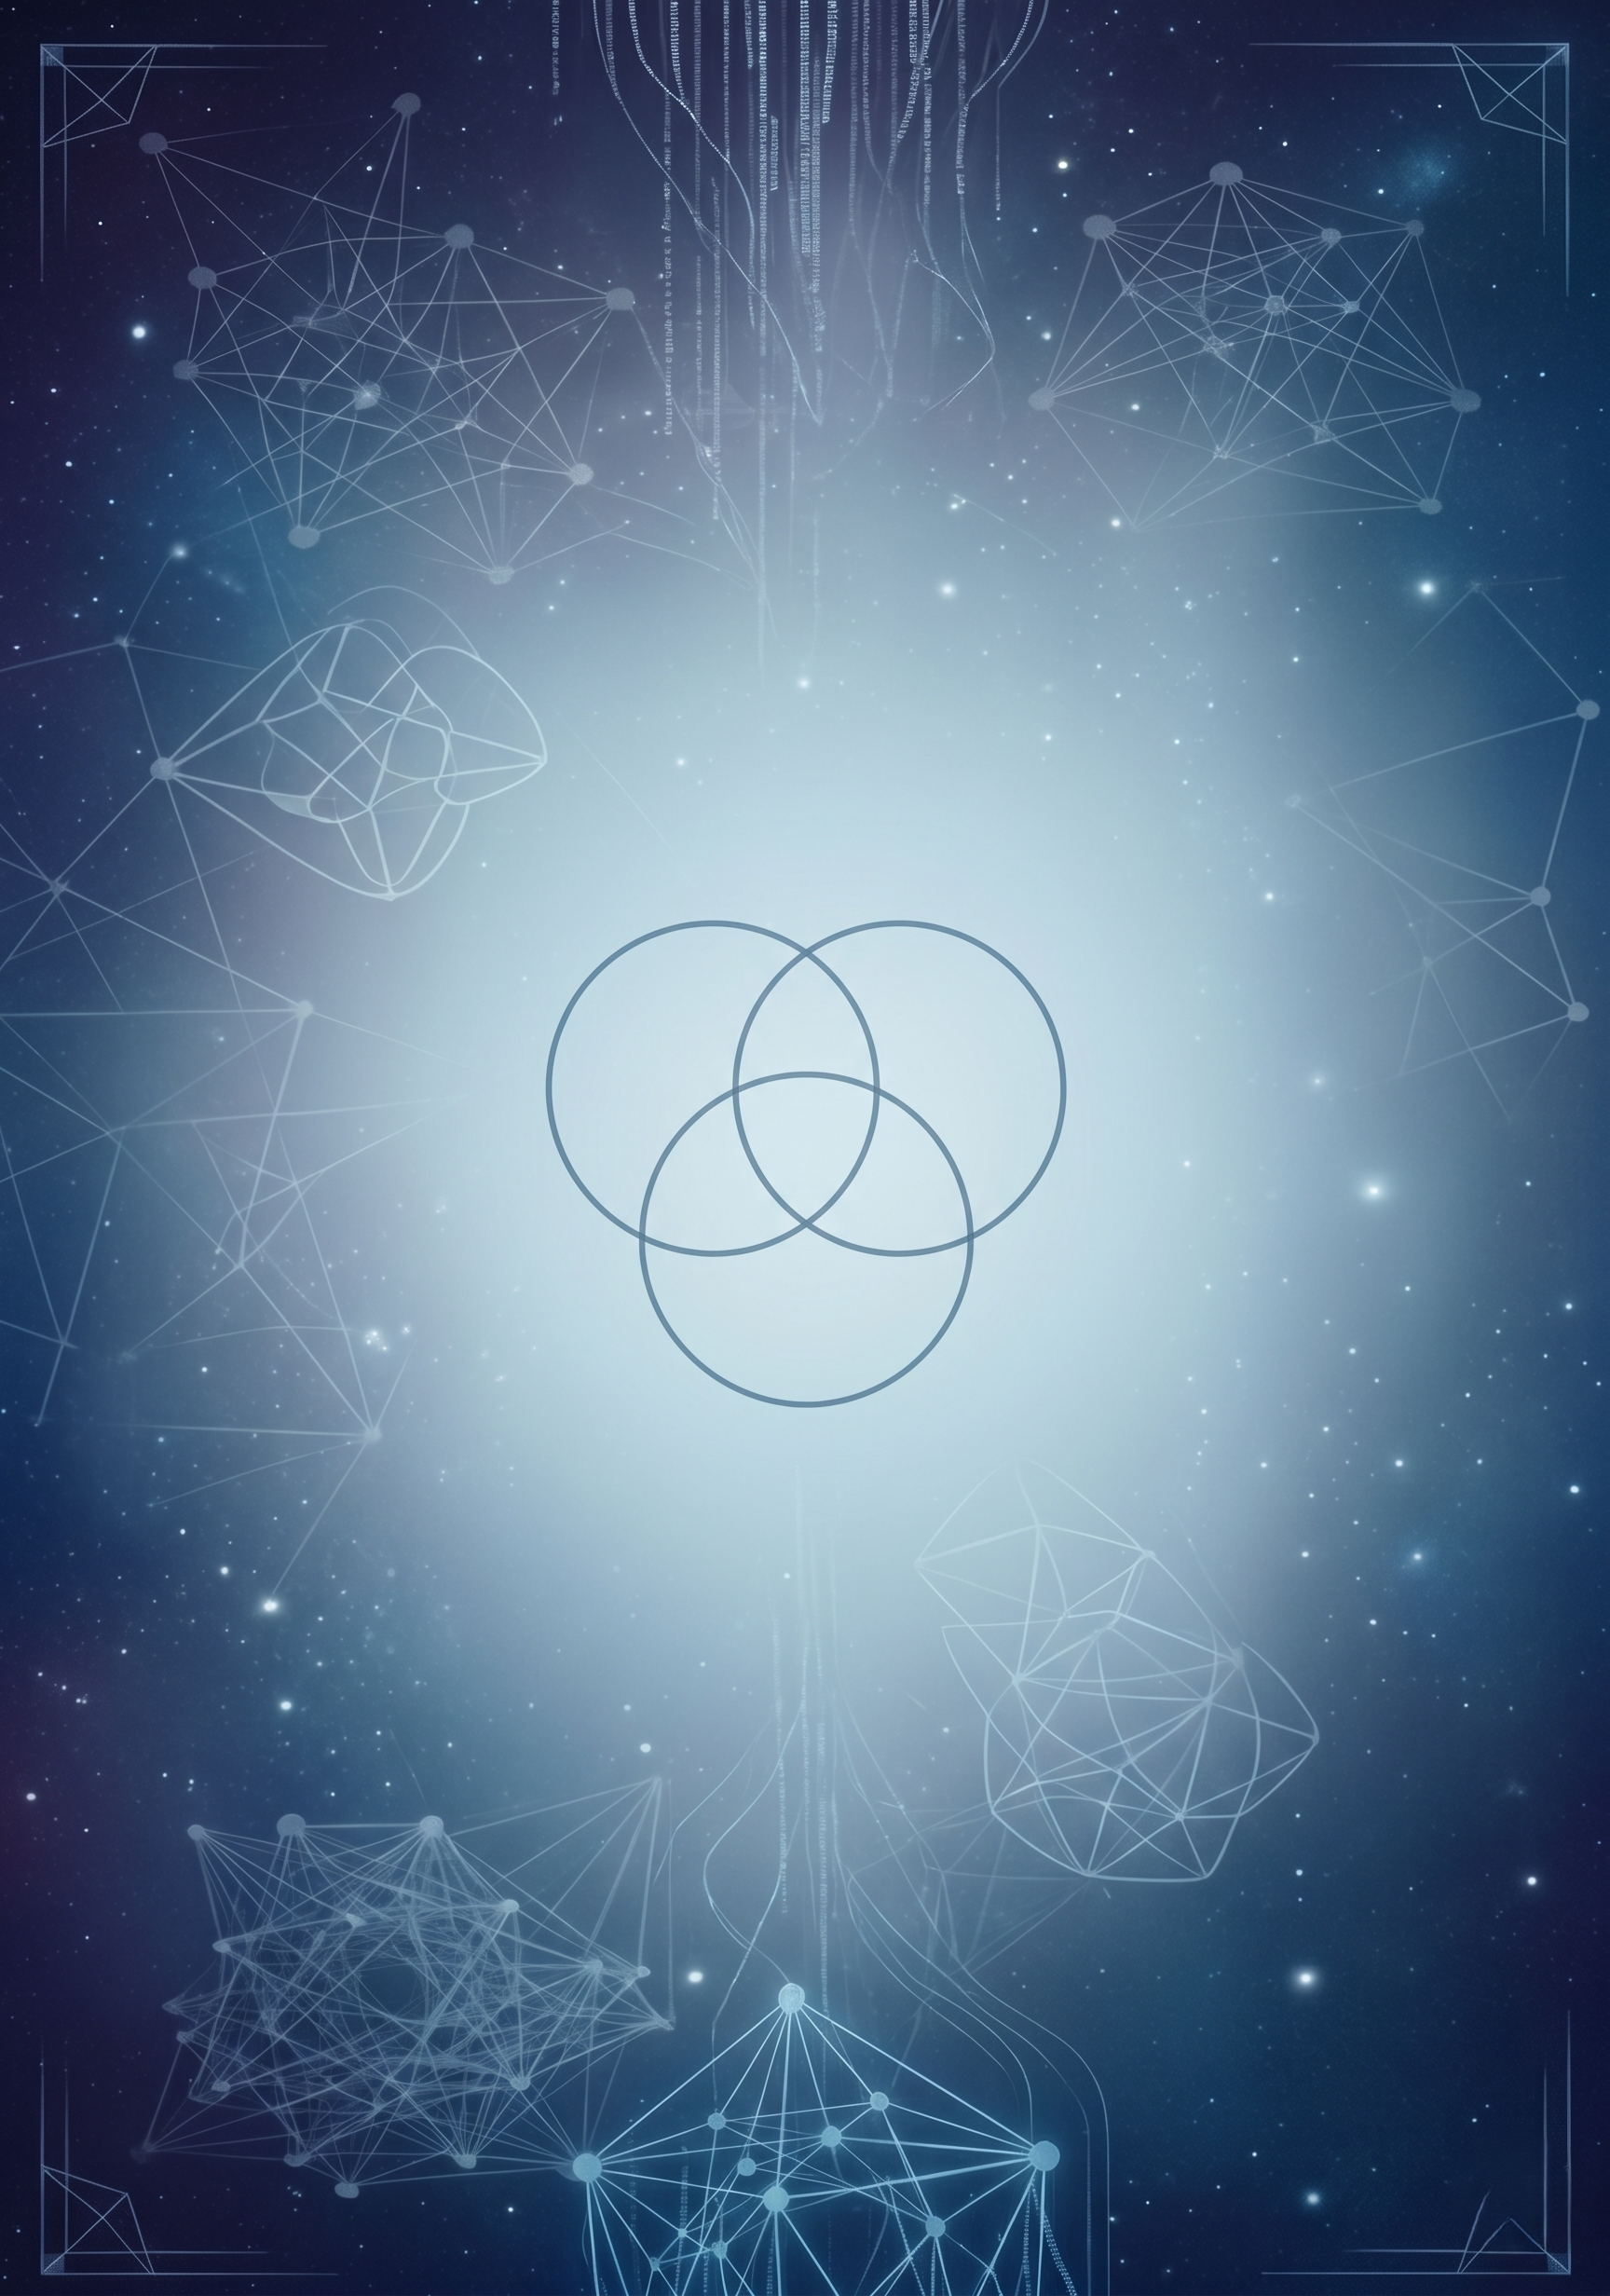
\includegraphics[width=\paperwidth, height=\paperheight]{figures/front_page.png}
        };
    \end{tikzpicture}

    \vspace*{6cm}
    \begin{center}
    \begin{tcolorbox}[enhanced, colback=white!90!black, colframe=primary, arc=8pt,
        width=0.85\textwidth, halign=center, boxsep=15pt, drop shadow]

        {\Huge \textbf{\color{primary} Probabilistic Methods}\par}
        \vspace{0.8cm}
        {\Large An Expanded Treatise on Theoretical \& Algorithmic Applications\par}
        \vspace{1.5cm}
        {\Large \textit{Sanidhya Saraf}\par}
        \vspace{0.5cm}

    \end{tcolorbox}
    \end{center}
\end{titlepage}

\tableofcontents
\newpage

% =====================================================================
%  MAIN CONTENT
% =====================================================================
% =====================================================================
%  Chapter 1 — Introduction: The Probabilistic Method
%  File: chapters/01_introduction.tex
%  Restyled to match Chapter 2 (boxed environments + Insight callouts).
%  Labels needed by later chapters are preserved (notably thm:szele and
%  the method of conditional expectations).
% =====================================================================
\providecommand{\E}{\mathbb{E}}
\providecommand{\Prob}{\mathbb{P}}
\providecommand{\ind}{\mathbf{1}}

\chapter{The Probabilistic Method}
\label{chap:intro}

The probabilistic method is a technique for proving that an object exists by
showing that a \emph{random} object has the desired property with positive
probability. One never points to the object; one merely argues that the
alternative --- that \emph{no} good object exists --- would force a
probability to be zero when it cannot be. The disorienting feature, the first
time one meets it, is that a question with no randomness in its statement is
answered by introducing randomness that the answer then discards.

Two facts do almost all the work in this chapter. The first is \emph{linearity
of expectation}, $\E[\sum_i X_i]=\sum_i\E[X_i]$, valid with no independence
assumption; the second is the \emph{union bound},
$\Prob(\bigcup_i E_i)\le\sum_i\Prob(E_i)$. From these we extract existence
through one elementary principle: if $\E[X]=\mu$ then some outcome has
$X\ge\mu$ and some has $X\le\mu$, and if $\Prob(\bigcup_i E_i)<1$ then some
outcome avoids every $E_i$. The rest of the chapter is variations on this
theme, sharpened twice --- by \emph{alteration} (fix the defects of a random
object) and by the \emph{Lov\'asz Local Lemma} (escape the union bound when
dependencies are sparse).

% =====================================================================
\section{A first example: large bipartite subgraphs}
% =====================================================================

\begin{theorem}{Large bipartite subgraph}{maxcut}
Every graph with $m$ edges contains a bipartite subgraph with at least $m/2$
edges.
\end{theorem}

\begin{proof}
Colour each vertex of $G=(V,E)$ black or white, independently and uniformly at
random, and let $E'$ be the set of edges joining opposite colours. The graph
$(V,E')$ is bipartite by construction. Each edge lands in $E'$ exactly when its
two endpoints receive different colours, which happens with probability
$1/2$, so by linearity $\E|E'|=\tfrac12|E|$. Some colouring therefore achieves
$|E'|\ge\tfrac12|E|$, and that colouring exhibits the required subgraph.
\end{proof}

\begin{insight}
This is the probabilistic method in miniature, and worth dwelling on because
every later argument is a descendant. Note what the proof does \emph{not} do:
it never produces a good bipartition, only certifies one exists. The bound
$m/2$ is also a genuine guarantee, not just an asymptotic --- and it is
essentially tight, since the complete graph $K_n$ has $\binom n2$ edges but its
largest cut has only $\lfloor n^2/4\rfloor\approx m/2$ of them. Read
algorithmically, the same statement says random colouring is a
$\tfrac12$-approximation for \textsc{Max-Cut}; the entire field of randomized
approximation grows from exactly this observation.
\end{insight}

% =====================================================================
\section{From existence to algorithm}
% =====================================================================

A first-moment proof asserts existence but offers no recipe. Often one can be
recovered, by replacing a single random choice for the whole object with a
sequence of \emph{conditional} choices.

\begin{remark}{The method of conditional expectations}{condexp}
Instead of colouring all vertices of $G$ at once, colour them one at a time. At
vertex $v_k$, the colours of $v_1,\dots,v_{k-1}$ are already fixed; compute the
conditional expectation of $|E'|$ under each of the two choices for $v_k$
(with the remaining vertices still random) and commit to whichever is larger.
Because the average of the two conditional expectations equals the expectation
before the choice, the running conditional expectation never decreases. It
starts at $m/2$ and ends, once all vertices are coloured, at the actual cut
size --- which is therefore at least $m/2$. The existence proof has become a
deterministic linear-time algorithm.
\end{remark}

The same idea is a workhorse in theoretical computer science. Consider
\textsc{Max-Sat}: given a boolean formula in conjunctive normal form, satisfy
as many clauses as possible.

\begin{theorem}{Expected satisfiability}{maxsat}
A CNF formula with $m$ clauses, where clause $C_j$ has $k_j$ distinct literals,
admits a truth assignment satisfying at least
$\displaystyle\sum_{j=1}^m\bigl(1-2^{-k_j}\bigr)$ clauses.
\end{theorem}

\begin{proof}
Set each variable to true or false independently with probability $1/2$. Clause
$C_j$ fails only if all $k_j$ of its literals evaluate to false, an event of
probability $2^{-k_j}$ by independence, so the indicator $Z_j$ of ``$C_j$
satisfied'' has $\E[Z_j]=1-2^{-k_j}$. Linearity gives
$\E\sum_j Z_j=\sum_j(1-2^{-k_j})$, and some assignment meets this average.
\end{proof}

\begin{insight}
For clauses of width $k_j\ge1$ this guarantees at least $m/2$ satisfied
clauses, and the bound improves as clauses lengthen --- width-$3$ clauses
alone already force a $\tfrac78$ fraction. Derandomized by conditional
expectations, this is Johnson's algorithm. The right way to see conditional
expectations is as a \emph{potential function}: the conditional mean is a
quantity you can always hold steady or raise by a local decision, so a greedy
walk down the tree of choices lands at an outcome no worse than the global
average. That reframing --- existence proof as potential function ---
recurs throughout combinatorial optimization.
\end{insight}

% =====================================================================
\section{Counting Hamilton paths: Szele's theorem}
% =====================================================================

A \emph{tournament} is an orientation of $K_n$, and a \emph{Hamilton path} is a
directed path through all $n$ vertices. The following 1943 result is often
called the first true application of the probabilistic method.

\begin{theorem}{Szele 1943}{szele}
There is a tournament on $n$ vertices with at least $\dfrac{n!}{2^{\,n-1}}$
Hamilton paths.
\end{theorem}

\begin{proof}
Orient each edge of $K_n$ by an independent fair coin. Fix an ordering
$\pi=(v_1,\dots,v_n)$ of the vertices and let $X_\pi$ indicate that $\pi$ is a
directed path, i.e.\ that all $n-1$ consecutive edges point forward. These are
independent fair events, so $\Prob(X_\pi=1)=2^{-(n-1)}$. Summing over all $n!$
orderings, linearity gives $\E\sum_\pi X_\pi=n!\,2^{-(n-1)}$, and some
tournament attains at least the average.
\end{proof}

\begin{insight}
The proof is pure existence: it guarantees a tournament rich in Hamilton paths
without naming one. It is also a first taste of the first moment's habit of
being right in form but loose in scale --- the true maximum is exponentially
larger in its base, $n!/(2-o(1))^n$, a fact requiring much heavier machinery
(Alon's 1990 permanent bound). We return to the minimization side and these
sharper asymptotics in Chapter~2; here Szele serves simply as the historical
seed of everything that follows.
\end{insight}

% =====================================================================
\section{Lower bounds for Ramsey numbers}
% =====================================================================

\begin{definition}{Ramsey number}{ramseynum}
The \emph{Ramsey number} $R(k,\ell)$ is the least $n$ such that every red/blue
edge-colouring of $K_n$ contains a red $K_k$ or a blue $K_\ell$. Ramsey (1929)
proved $R(k,\ell)$ is finite; for instance $R(3,3)=6$.
\end{definition}

\begin{remark}{A historical aside}{history}
Paul Erd\H{o}s (1913--1996), with roughly $1{,}500$ papers and over $500$
collaborators, is regarded as the father of the probabilistic method; the
Ramsey lower bound below comes from his 1947 paper. Frank Ramsey (1903--1930)
did foundational work in logic, philosophy, and economics before dying at
$26$. Because so much of the subject traces to Erd\H{o}s's circle, Hungarian
names abound; a pronunciation guide:
\begin{center}\small
\begin{tabular}{lll}
\toprule
\textbf{Spelling} & \textbf{Sounds like} & \textbf{Examples}\\
\midrule
s  & sh & Erd\H{o}s, Simonovits\\
sz & s  & Szemer\'edi, Lov\'asz\\
\bottomrule
\end{tabular}
\end{center}
\end{remark}

\begin{theorem}{Erd\H{o}s 1947}{ramsey1}
If $\binom nk 2^{\,1-\binom k2}<1$, then $R(k,k)>n$.
\end{theorem}

\begin{proof}
Colour the edges of $K_n$ red/blue independently and uniformly. For each
$k$-set $S$ let $A_S$ be the event that $S$ is monochromatic; the
$\binom k2$ edges inside $S$ must agree, so $\Prob(A_S)=2^{\,1-\binom k2}$. By
the union bound,
\[
  \Prob\Bigl(\textstyle\bigcup_S A_S\Bigr)
  \le \sum_{S}\Prob(A_S)=\binom nk 2^{\,1-\binom k2}<1,
\]
so with positive probability no $A_S$ occurs --- a colouring with no
monochromatic $K_k$.
\end{proof}

\begin{remark}{Quantitative form}{ramsey1q}
Optimizing $n$ via Stirling gives
$R(k,k)>\bigl(\tfrac{1}{e\sqrt2}+o(1)\bigr)k\,2^{k/2}$. From the other side,
Erd\H{o}s--Szekeres (1935) showed $R(k,k)\le(4-o(1))^k$, and Campos,
Griffiths, Morris, and Sahasrabudhe (2023+) achieved the first exponential
improvement, $R(k,k)\le(4-c)^k$ for some $c>0$.
\end{remark}

\begin{insight}
The union bound is nothing but the first moment in disguise: $\sum_S\Prob(A_S)$
is the \emph{expected} number of monochromatic cliques, and ``expected number
$<1$'' forces ``some outcome has zero.'' The proof is also the standard
illustration of existence without construction --- a random colouring works
with overwhelming probability, yet no efficient way is known to certify that a
given colouring is good, a situation memorably described as finding hay in a
haystack. Pinning down an explicit construction matching the random bound is a
deep open problem with surprising ties to randomness extractors.
\end{insight}

\subsection*{Alteration}

\begin{theorem}{Ramsey lower bound via alteration}{ramsey_alt}
For all $k,n$, $\;R(k,k)>n-\binom nk 2^{\,1-\binom k2}$.
\end{theorem}

\begin{proof}
Colour $K_n$ at random as before, then \emph{delete} one vertex from each
monochromatic $K_k$; the result has no monochromatic $K_k$. If $X$ counts the
monochromatic cliques after step one, then $\E[X]=\binom nk 2^{\,1-\binom k2}$,
and we remove at most $X$ vertices, leaving at least $n-X$ with expectation
$n-\binom nk 2^{\,1-\binom k2}$. Some outcome meets this expectation.
\end{proof}

\begin{remark}{}{ramsey_altq}
Optimizing $n$ yields $R(k,k)>\bigl(\tfrac1e+o(1)\bigr)k\,2^{k/2}$, a factor
$\sqrt2$ better than the union-bound estimate.
\end{remark}

\begin{insight}
Alteration --- also called the deletion method --- is the first genuine upgrade
to the bare first moment: rather than demanding that a random object be perfect,
we accept a flawed one and pay to repair it. The accounting is the same first
moment, now applied to the \emph{cost of repair} (the expected number of
deletions) rather than to success outright. The payoff here is only a constant
factor, but the pattern --- build sloppily, then clean up --- is one of the
most broadly useful in the subject.
\end{insight}

\subsection*{The Lov\'asz Local Lemma}

To avoid bad events $E_1,\dots,E_m$ there are two crude regimes. The union
bound needs $\sum_i\Prob(E_i)<1$, which collapses once the events are
numerous. Full independence gives
$\Prob(\bigcap_i \overline{E_i})=\prod_i(1-\Prob(E_i))>0$, but genuine
independence is rare. The local lemma occupies the ground between: sparse
dependence suffices.

\begin{theorem}{Lov\'asz Local Lemma (variable model)}{lll}
Let $x_1,\dots,x_N$ be independent random variables and
$B_1,\dots,B_m\subseteq[N]$, with each event $E_i$ determined by
$\{x_j:j\in B_i\}$. If every $B_i$ meets at most $d$ other $B_j$ and
$\Prob(E_i)\le\dfrac{1}{(d+1)e}$ for all $i$, then with positive probability
none of the $E_i$ occur. (The constant $e$ is optimal; proof deferred to
Chapter~6.)
\end{theorem}

\begin{theorem}{Spencer 1977}{ramsey_lll}
If $\;e\bigl(\binom k2\binom{n}{k-2}+1\bigr)2^{\,1-\binom k2}\le 1$, then
$R(k,k)>n$.
\end{theorem}

\begin{proof}
Colour $K_n$ at random, one independent variable per edge, and let $E_S$ be the
event that the $k$-set $S$ is monochromatic, so $\Prob(E_S)=2^{\,1-\binom k2}$.
Two cliques share an edge precisely when their vertex sets overlap in at least
two vertices, and each $S$ has at most $\binom k2\binom{n}{k-2}$ such partners.
With $d=\binom k2\binom{n}{k-2}$, the hypothesis is exactly the local-lemma
condition $\Prob(E_S)\le 1/((d+1)e)$, so positively often no $E_S$ occurs.
\end{proof}

\begin{remark}{}{ramsey_lllq}
Optimizing gives $R(k,k)>\bigl(\tfrac{\sqrt2}{e}+o(1)\bigr)k\,2^{k/2}$, the best
lower bound known.
\end{remark}

\begin{insight}
The three Ramsey bounds form a clean ladder, each rung a factor $\sqrt2$ above
the last:
\[
  \tfrac{1}{e\sqrt2}\ \xrightarrow{\text{union bound}}\
  \tfrac{1}{e}\ \xrightarrow{\text{alteration}}\
  \tfrac{\sqrt2}{e}\ \ (k\,2^{k/2}).
\]
It is the same problem solved three times with progressively sharper tools, and
a faithful map of the method's hierarchy --- first moment, then repair, then
local independence. Tellingly, decades of effort have not moved the
\emph{leading constant} past $\sqrt2/e$ from below, even as the upper bound has
only recently cracked $4^k$ from above; the multiplicative gap in
$R(k,k)^{1/k}$ between $\sqrt2$ and $4-c$ remains one of the famous open
problems of the area.
\end{insight}

% =====================================================================
\section{Extremal set systems}
% =====================================================================

A set family $\mathcal F$ on ground set $[n]$ is an \emph{antichain} if no
member contains another. The extremal question --- how large can an antichain
be --- has a one-line probabilistic answer.

\begin{theorem}{Sperner 1928}{sperner}
An antichain of subsets of $[n]$ has at most $\binom{n}{\lfloor n/2\rfloor}$
members.
\end{theorem}

This follows from a stronger weighted statement.

\begin{theorem}{LYM inequality}{lym}
For an antichain $\mathcal F\subseteq 2^{[n]}$,
$\displaystyle\sum_{A\in\mathcal F}\binom{n}{|A|}^{-1}\le 1.$
\end{theorem}

\begin{proof}
Draw a uniform random permutation $\sigma$ of $[n]$ and form the maximal chain
$\emptyset\subset\{\sigma(1)\}\subset\{\sigma(1),\sigma(2)\}\subset\cdots\subset[n]$.
A fixed set $A$ appears in this chain exactly when $\sigma$ lists the elements
of $A$ first (in some order) and then the rest, which happens for
$|A|!\,(n-|A|)!$ of the $n!$ permutations; hence
$\Prob(A\in\text{chain})=\binom{n}{|A|}^{-1}$. The chain is itself a chain, so
it contains at most one member of the antichain $\mathcal F$ --- the events
``$A\in\text{chain}$'' for $A\in\mathcal F$ are disjoint, and their
probabilities sum to at most $1$.
\end{proof}

Sperner's bound drops out, since $\binom{n}{|A|}\le\binom{n}{\lfloor n/2\rfloor}$
makes each term at least $\binom{n}{\lfloor n/2\rfloor}^{-1}$, so
$|\mathcal F|\le\binom{n}{\lfloor n/2\rfloor}$.

\begin{insight}
The trick is a normalization: a uniformly random maximal chain meets each set
$A$ with probability $1/\binom{n}{|A|}$, so weighting each set by that
reciprocal turns the geometric fact ``a chain hits an antichain at most once''
into the analytic inequality $\sum 1/\binom{n}{|A|}\le1$. It is again a
first-moment argument, this time bounding the expected number of hits ($\le1$)
from above; equality forces $\mathcal F$ to be a single middle layer. The same
random-ordering device, suitably adapted, proves the next two theorems too ---
it is the unifying engine of probabilistic extremal set theory.
\end{insight}

\begin{theorem}{Bollob\'as two families theorem 1965}{bollobas}
Let $A_1,\dots,A_m$ and $B_1,\dots,B_m$ be finite sets with $A_i\cap B_i=\emptyset$
for all $i$ and $A_i\cap B_j\ne\emptyset$ for all $i\ne j$. Then
$\displaystyle\sum_{i=1}^m\binom{|A_i|+|B_i|}{|A_i|}^{-1}\le 1.$
\end{theorem}

\begin{proof}
Take a uniform random ordering of $\bigcup_i(A_i\cup B_i)$ and let $E_i$ be the
event that every element of $A_i$ precedes every element of $B_i$. Restricted
to $A_i\cup B_i$, this asks the $|A_i|$ elements of $A_i$ to come first among
$|A_i|+|B_i|$, so $\Prob(E_i)=\binom{|A_i|+|B_i|}{|A_i|}^{-1}$. The events are
pairwise disjoint: if $E_i$ and $E_j$ both held, the disjointness and crossing
hypotheses on $A_i,B_i,A_j,B_j$ would be contradicted. Disjoint events sum to
at most $1$.
\end{proof}

\begin{remark}{Why it is natural: transversals}{bollobastrans}
The uniform case $|A_i|=r,\,|B_i|=s$ reads $m\le\binom{r+s}{r}$, and it is
sharp. It also answers a question about transversals. Call $T$ a
\emph{transversal} of a family if it meets every member, write $\tau$ for the
minimum transversal size, and call a family $\tau$-critical if deleting any
member lowers $\tau$. The largest $\tau$-critical $r$-uniform family with
$\tau=s+1$ has exactly $\binom{r+s}{r}$ members: take the $A_i$ as the sets and
$B_i$ as an $s$-element transversal of the family with $A_i$ removed, and the
hypotheses of the theorem hold. Sperner and LYM are themselves special cases,
via $B_i=[n]\setminus A_i$.
\end{remark}

A family is \emph{intersecting} if any two of its members meet.

\begin{theorem}{Erd\H{o}s--Ko--Rado 1961}{ekr}
If $n\ge 2k$, an intersecting family of $k$-subsets of $[n]$ has at most
$\binom{n-1}{k-1}$ members.
\end{theorem}

\begin{proof}
Arrange $1,\dots,n$ uniformly at random around a circle and call a $k$-set
\emph{contiguous} if it forms an arc. A fixed $k$-set is contiguous with
probability $n/\binom nk$, so the expected number of contiguous members of
$\mathcal F$ is $n|\mathcal F|/\binom nk$. On the other hand, any single
circular arrangement contains at most $k$ contiguous members of an intersecting
family: fixing one contiguous member $A$, the only arcs meeting $A$ come in
disjoint pairs once $n\ge 2k$, so at most $k$ of them (including $A$) can
pairwise intersect. Hence $n|\mathcal F|/\binom nk\le k$, giving
$|\mathcal F|\le\tfrac kn\binom nk=\binom{n-1}{k-1}$.
\end{proof}

\begin{insight}
This is Katona's \emph{cycle method}: average over rotations rather than over
subsets, so a global counting problem becomes a tiny local one --- how many
arcs of an intersecting family fit on one circle. The hypothesis $n\ge2k$ is
not cosmetic; for $n<2k$ \emph{every} pair of $k$-sets intersects by
pigeonhole, the family $\binom{[n]}{k}$ is itself intersecting, and the bound
fails. The extremal family --- all $k$-sets through a fixed element --- shows
the answer $\binom{n-1}{k-1}$ is exactly right.
\end{insight}

% =====================================================================
\section{Two-colourable hypergraphs}
% =====================================================================

A $k$-uniform hypergraph is \emph{$2$-colourable} (has \emph{property B}) if its
vertices can be coloured with two colours leaving no edge monochromatic. Let
$m(k)$ be the fewest edges in a $k$-uniform hypergraph that is \emph{not}
$2$-colourable. The first values are $m(2)=3$, $m(3)=7$ (the Fano plane), and
$m(4)=23$ (found by computer search); $m(k)$ is unknown for every $k\ge5$. The
probabilistic method brackets it from both sides.

\begin{theorem}{Lower bound, Erd\H{o}s 1964}{hyper_lower}
$m(k)\ge 2^{k-1}$ for every $k\ge2$.
\end{theorem}

\begin{proof}
Suppose the hypergraph has $m<2^{k-1}$ edges and colour the vertices with a
uniform random $2$-colouring. A fixed $k$-edge is monochromatic with
probability $2\cdot 2^{-k}=2^{-(k-1)}$, so the expected number of monochromatic
edges is at most $2^{-(k-1)}m<1$. Some colouring therefore has none, i.e.\ the
hypergraph is $2$-colourable.
\end{proof}

\begin{theorem}{Upper bound, Erd\H{o}s 1964}{hyper_upper}
$m(k)=O(k^2 2^k)$.
\end{theorem}

\begin{proof}
Put $n=k^2$ vertices and build $H$ by choosing $m$ edges uniformly at random
(with replacement) from all $k$-subsets. Fix a $2$-colouring splitting the
vertices into parts of sizes $a$ and $b=n-a$. A random edge avoids being
monochromatic unless it lands entirely in one part, and a short estimate gives
$\Prob(\text{edge monochromatic})\ge c\,2^{-k}$ for an absolute $c>0$. The $m$
edges are independent, so
\[
  \Prob(\chi\text{ is proper})\le(1-c\,2^{-k})^m\le e^{-c\,2^{-k}m},
\]
and a union bound over all $2^n$ colourings gives
$\Prob(H\text{ is }2\text{-colourable})\le 2^n e^{-c\,2^{-k}m}<1$ once
$m=O(k^2 2^k)$ (recall $n=k^2$). Some such $H$ is then non-$2$-colourable.
\end{proof}

\begin{insight}
These two proofs run the probabilistic method in opposite directions. The lower
bound shows a \emph{good} object exists (a proper colouring) by making the
expected number of defects small. The upper bound shows a \emph{bad} object
exists (a non-colourable hypergraph) by making every fixed colouring likely to
fail and union-bounding over all colourings. Recognizing which direction a
problem wants --- existence of structure versus existence of a hard instance ---
is half the battle. The current record narrows the gap to
$m(k)\gtrsim 2^k\sqrt{k/\log k}$, still proved probabilistically.
\end{insight}

% =====================================================================
\section{The list chromatic number of \texorpdfstring{$K_{n,n}$}{Knn}}
% =====================================================================

In \emph{list colouring}, every vertex receives its own list of allowed colours;
$G$ is \emph{$k$-choosable} if a proper colouring exists for \emph{every}
assignment of $k$-element lists, and the \emph{list chromatic number}
$\mathrm{ch}(G)$ is the least such $k$. Always $\chi(G)\le\mathrm{ch}(G)$, and
the gap can be large: $K_{3,3}$ is $2$-colourable but not $2$-choosable.

\begin{theorem}{Upper bound}{list_upper}
If $n<2^{k-1}$ then $K_{n,n}$ is $k$-choosable; equivalently
$\mathrm{ch}(K_{n,n})\le\lfloor\log_2(2n)\rfloor+1$.
\end{theorem}

\begin{proof}
Mark each colour ``L'' or ``R'' by an independent fair coin. On a left vertex,
discard the colours marked R; on a right vertex, discard those marked L. A
fixed vertex loses its whole list of size $k$ with probability $2^{-k}$, so by
the union bound some vertex is emptied with probability at most $2n\,2^{-k}<1$.
With positive probability every list keeps a colour, and since left and right
vertices now draw from disjoint colour pools (L versus R), assigning any
surviving colour is proper.
\end{proof}

\begin{theorem}{Lower bound}{list_lower}
If some non-$2$-colourable $k$-uniform hypergraph has $n$ edges, then $K_{n,n}$
is not $k$-choosable.
\end{theorem}

\begin{proof}
Let $H$ be such a hypergraph with edges $e_1,\dots,e_n$ and treat its vertices
as colours. Give the $i$-th left vertex and the $i$-th right vertex the list
$e_i$. A proper list colouring would pick one colour (vertex of $H$) per list
(edge of $H$); the left choices and right choices each induce a colour class
that must hit every edge, forcing a proper $2$-colouring of $H$ --- which does
not exist.
\end{proof}

Combining the two with the hypergraph bound $m(k)=O(k^2 2^k)$ gives the
asymptotics.

\begin{corollary}{}{list_cor}
$\mathrm{ch}(K_{n,n})=(1+o(1))\log_2 n.$
\end{corollary}

\begin{insight}
The lower bound is the striking half: list-colourability of a graph is governed
by a $2$-colourability question about a hypergraph, so the difficulty of
property B transfers wholesale to choosability. Unlike the ordinary chromatic
number, $\mathrm{ch}$ keeps growing with average degree --- Saxton and Thomason
(2015) proved $\mathrm{ch}(G)>(1+o(1))\log_2 d$ for average degree $d$, with
$K_{n,n}$ showing this is sharp, via the method of \emph{hypergraph
containers}, one of the major modern developments in the area.
\end{insight}

% =====================================================================
\section*{Exercises}
\addcontentsline{toc}{section}{Exercises}
% =====================================================================

\begin{enumerate}[itemsep=4pt]
  \item Verify the asymptotic calculations behind the Ramsey lower bounds:
        \begin{enumerate}
          \item the largest $n$ with $\binom nk 2^{1-\binom k2}<1$ is
                $\bigl(\tfrac{1}{e\sqrt2}+o(1)\bigr)k\,2^{k/2}$;
          \item the maximum of $n-\binom nk 2^{1-\binom k2}$ over $n$ is
                $\bigl(\tfrac1e+o(1)\bigr)k\,2^{k/2}$;
          \item the largest $n$ with
                $e(\binom k2\binom{n}{k-2}+1)2^{1-\binom k2}<1$ is
                $\bigl(\tfrac{\sqrt2}{e}+o(1)\bigr)k\,2^{k/2}$.
        \end{enumerate}
  \item Prove that if some $p\in[0,1]$ satisfies
        $\binom nk p^{\binom k2}+\binom nt(1-p)^{\binom t2}<1$, then
        $R(k,t)>n$. Deduce $R(4,t)\ge c\,(t/\log t)^{3/2}$.
  \item Let $G$ have $n$ vertices and $m$ edges. Prove $K_n$ is a union of
        $O(n^2(\log n)/m)$ isomorphic copies of $G$ (not necessarily
        edge-disjoint).
  \item Prove there is an absolute $C>0$ such that every $n\times n$ matrix with
        distinct real entries can have its rows permuted so that no column
        contains an increasing subsequence of length $\ge C\sqrt n$.
  \item (Generalized Sperner.) If $\mathcal F\subseteq 2^{[n]}$ contains no
        chain $A_1\subsetneq\cdots\subsetneq A_{k+1}$, prove $|\mathcal F|$ is at
        most the union of the $k$ middle layers of the Boolean lattice.
  \item Let $G$ have $n\ge10$ vertices and suppose adding any edge creates a new
        $K_{10}$. Prove $G$ has at least $8n-36$ edges. \textit{(Hint: Bollob\'as.)}
  \item Let $k\ge4$ and let $H$ be a $k$-uniform hypergraph with at most
        $4^{k-1}/3^k$ edges. Prove its vertices can be $4$-coloured so that
        every edge sees all four colours.
  \item For $\mathcal F\subseteq 2^{[n]}$ and $A\subseteq[n]$ write
        $\mathcal F|_A=\{S\cap A:S\in\mathcal F\}$. Prove that for every $n,k$
        there is $\mathcal F$ with $|\mathcal F|=O(k2^k\log n)$ such that
        $\mathcal F|_A=2^A$ for every $k$-set $A$.
  \item Let $A_i$ be $r$-sets and $B_i$ be $s$-sets with $A_i\cap B_i=\emptyset$,
        and for each $i\ne j$ at least one of $A_i\cap B_j$, $A_j\cap B_i$
        nonempty. Prove $m\le(r+s)^{r+s}/(r^r s^s)$.
  \item $\bigstar$ Show that every non-$2$-colourable $n$-uniform hypergraph has
        at least $\tfrac n2\binom{2n-1}{n}$ unordered pairs of edges meeting in
        exactly one vertex.
\end{enumerate}

% =====================================================================
%  Chapter 2 — Linearity of Expectation
%  File: chapters/02_linearity.tex
%  Built from the handout; deliberately avoids material already covered
%  in Chapter 1 (notably the full proof of Szele's theorem and the
%  general method of conditional expectations).
% =====================================================================
\providecommand{\E}{\mathbb{E}}
\providecommand{\Prob}{\mathbb{P}}
\providecommand{\ind}{\mathbf{1}}
\providecommand{\cross}{\operatorname{cr}}

\chapter{Linearity of Expectation}
\label{chap:linearity}

In Chapter~1 we used the first moment mostly as a switch that turns ``positive
probability'' into ``existence.'' This chapter develops the same idea into a
quantitative instrument. The engine throughout is a single identity: for
random variables $X_1,\dots,X_n$ and scalars $c_1,\dots,c_n$,
\[
  \E\!\Big[\textstyle\sum_i c_i X_i\Big] = \sum_i c_i\,\E[X_i].
\]
Its decisive feature is what it omits --- there is \emph{no independence
hypothesis}. Expectation is an integral against the probability measure, and
integrals are linear regardless of how their summands interact. Products
enjoy no such luxury: $\E[XY]=\E[X]\,\E[Y]$ holds only when $X$ and $Y$ are
uncorrelated, and independence is merely a sufficient condition for that.

We pair the identity with one elementary observation, used so often that it
deserves a name.

\begin{proposition}{The averaging principle}{averaging}
For any random variable $X$ with finite mean, there is an outcome with
$X\ge\E[X]$ and an outcome with $X\le\E[X]$.
\end{proposition}

\begin{proof}
If $X<\E[X]$ held on the whole sample space, then taking expectations of both
sides would give $\E[X]<\E[X]$, a contradiction; symmetrically for the other
inequality.
\end{proof}

The recipe for the rest of the chapter is fixed: build a random object, write
the quantity of interest as a sum of simple indicators, evaluate the
expectation by linearity, and invoke the averaging principle to extract a
single good outcome.

\begin{insight}
The leverage is almost entirely in the \emph{decomposition}, not the
arithmetic. Whenever a global count splits as $X=\sum_i X_i$ with each
$\E[X_i]$ computable in isolation, linearity discards every correlation
between the $X_i$ at no cost. That is exactly why the method dominates
``average case'' counting: the dependence that defeats exact enumeration is
invisible to the first moment. The same blindness is the method's limitation
--- it locates the mean but says nothing about concentration, which is the
job of the second moment (Chapter~3).
\end{insight}

% =====================================================================
\section{Warm-up: fixed points of a random permutation}
% =====================================================================

\begin{question}{Expected number of fixed points}{fixedpoints}
What is the average number of fixed points of a uniformly random permutation
of an $n$-element set?
\end{question}

\begin{proof}[Solution]
Let $X_i$ be the indicator of the event $\pi(i)=i$, where $\pi$ is uniform on
the symmetric group. A uniform permutation sends $i$ to each position with
probability $1/n$, so $\E[X_i]=\Prob(\pi(i)=i)=1/n$. The number of fixed
points is $X_1+\cdots+X_n$, and by linearity
\[
  \E[X_1+\cdots+X_n] = \sum_{i=1}^n \E[X_i] = n\cdot\frac1n = 1,
\]
independent of $n$.
\end{proof}

\begin{insight}
The exact answer $1$, free of any error term, is the signature of linearity
ignoring dependence: the $X_i$ are strongly correlated (fixing many points
constrains the rest), yet none of that surfaces. The structure underneath is
richer still. As $n\to\infty$ the number of fixed points converges to a
$\mathrm{Poisson}(1)$ law, so the probability of \emph{no} fixed point tends
to $e^{-1}$ --- the classical derangement constant. A variance computation
gives $\operatorname{Var}=1$ as well, so the mean of $1$ is genuinely
informative rather than washed out by spread.
\end{insight}

% =====================================================================
\section{Hamilton paths in tournaments}
% =====================================================================

\begin{definition}{Tournament and Hamilton path}{tournament}
A \emph{tournament} is an orientation of the complete graph $K_n$: between
every pair of vertices there is exactly one directed edge. A \emph{Hamilton
path} is a directed path that visits every vertex exactly once.
\end{definition}

\begin{question}{Extremes for Hamilton paths}{tourcount}
What are the maximum and the minimum possible numbers of Hamilton paths in an
$n$-vertex tournament?
\end{question}

\subsection*{The minimum}

The minimum is easy to pin down. The \emph{transitive} tournament, whose
edges respect a fixed linear order $v_1\to v_2\to\cdots\to v_n$, has exactly
one Hamilton path. No tournament can do worse:

\begin{proposition}{Every tournament has a Hamilton path}{everyhampath}
Every $n$-vertex tournament contains at least one Hamilton path.
\end{proposition}

\begin{proof}
Take a directed path $P=u_1\to u_2\to\cdots\to u_\ell$ of maximum length. If
some vertex $w$ is missing from $P$, consider the edge between $w$ and $u_1$:
if it points $w\to u_1$ we could prepend $w$, lengthening $P$. So it points
$u_1\to w$. Likewise the edge between $u_\ell$ and $w$ must point $w\to
u_\ell$, else we could append $w$. Walking along $P$, the orientation of the
edge between $w$ and $u_i$ thus switches from ``into $w$'' (at $i=1$) to ``out
of $w$'' (at $i=\ell$), so for some consecutive pair we have
$u_i\to w\to u_{i+1}$; inserting $w$ between $u_i$ and $u_{i+1}$ extends $P$,
contradicting maximality. Hence $P$ already covers all vertices.
\end{proof}

\subsection*{The maximum}

The maximization side is where the probabilistic method first appeared.
Szele's theorem, established in Chapter~1 (Theorem~\ref{thm:szele}), produces
a tournament with at least $n!\,/\,2^{n-1}$ Hamilton paths by orienting edges
with independent fair coins and averaging the path-indicators over all $n!$
orderings. We do not repeat that argument here; instead we record what
happens beyond it.

\begin{insight}
Szele's bound is a textbook example of the first moment being correct in
shape but loose in scale. Szele conjectured the true maximum to be
$n!\,/\,(2-o(1))^{n}$ --- exponentially larger \emph{in the base} than
$n!/2^{n-1}$. The first moment loses here precisely because it averages the
$n!$ path-indicators as if unrelated, when in fact orderings sharing many
edges rise and fall together. Closing the gap is genuinely harder: Alon
(1990) proved Szele's conjecture using the Minc--Br\'egman bound on
permanents, an entropy-flavoured estimate we return to in the chapter on the
entropy method. The lesson worth carrying: a first-moment existence proof is
a \emph{floor}, and the distance from that floor to the truth is often where
the substance lies.
\end{insight}

% =====================================================================
\section{Large sum-free subsets}
% =====================================================================

\begin{definition}{Sum-free set}{sumfree}
A subset $A$ of an abelian group is \emph{sum-free} if there are no
$a,b,c\in A$ (not necessarily distinct) with $a+b=c$.
\end{definition}

\begin{theorem}{Erd\H{o}s, 1965}{erdossumfree}
Every set of $n$ nonzero integers contains a sum-free subset of size at least
$n/3$.
\end{theorem}

\begin{proof}
Work on the circle $\mathbb{R}/\mathbb{Z}$, identified with $[0,1)$. The open
arc $(\tfrac13,\tfrac23)$ is itself sum-free there: if two of its points sum,
the result lands in $(\tfrac23,\tfrac43)\bmod 1$, which is disjoint from
$(\tfrac13,\tfrac23)$.

Let $A\subseteq\mathbb{Z}\setminus\{0\}$ with $|A|=n$. Pick $\theta\in[0,1]$
uniformly at random and set
\[
  A_\theta = \bigl\{\,a\in A : \{a\theta\}\in(\tfrac13,\tfrac23)\,\bigr\},
\]
where $\{\cdot\}$ is the fractional part. Since the dilation map preserves the
sum-free property, $A_\theta$ is sum-free for every $\theta$. For a fixed
nonzero integer $a$, the value $\{a\theta\}$ is uniform on $[0,1]$, so
$\Prob(a\in A_\theta)=\tfrac13$. By linearity, $\E\,|A_\theta|=n/3$, and the
averaging principle yields a $\theta$ with $|A_\theta|\ge n/3$.
\end{proof}

\begin{remark}{Sharper bounds}{sumfreesharper}
The constant can be nudged upward. Alon and Kleitman (1990) observed that
$A_\theta$ is empty for $\theta$ near $0$, so $|A_\theta|<n/3$ occurs with
positive probability; since $|A_\theta|$ is an integer, the bound improves to
$\ge(n+1)/3$. Bourgain (1997) reached $\ge(n+2)/3$ via a difficult Fourier
argument --- still the best known. Whether $\ge(n+f(n))/3$ holds with
$f(n)\to\infty$ is open. Conversely, Eberhard, Green, and Manners (2014)
constructed $n$-element sets whose largest sum-free subset has size at most
$(\tfrac13+o(1))n$, so the leading constant $1/3$ is correct.
\end{remark}

\begin{insight}
The number $1/3$ is not incidental: it is the measure of the largest sum-free
arc on the circle. So no choice of arc can beat $n/3$, which explains why the
celebrated lower-order improvements cannot come from tuning the construction
--- they must extract information about how the dilates $\{a\theta\}$
\emph{correlate} across different $a$, information the first moment throws
away by design.
\end{insight}

% =====================================================================
\section{Independent sets and Tur\'an's theorem}
% =====================================================================

We turn to extremal graph theory. The Tur\'an problem asks for the maximum
number of edges in an $n$-vertex $K_{r+1}$-free graph. By complementation this
is equivalent to forcing large \emph{independent} sets, and the following
degree-sensitive bound --- found independently by Caro (1979) and Wei (1981)
--- is the key.

\begin{theorem}{Caro 1979, Wei 1981}{carowei}
Every graph $G$ contains an independent set of size at least
$\displaystyle\sum_{v\in V(G)}\frac{1}{d_v+1}$, where $d_v=\deg v$.
\end{theorem}

\begin{proof}
Order the vertices uniformly at random and let $I$ be the set of vertices that
precede all of their neighbours in this order. Then $I$ is independent: if
adjacent $u,v$ both lay in $I$, each would have to precede the other. For a
fixed $v$, the event $v\in I$ is exactly that $v$ comes first among the
$d_v+1$ vertices of $\{v\}\cup N(v)$, which by symmetry has probability
$1/(d_v+1)$. Linearity gives $\E\,|I|=\sum_v 1/(d_v+1)$, and some ordering
attains at least this value.
\end{proof}

\begin{remark}{From randomness to a greedy algorithm}{caroweiderand}
This proof can be made constructive in the spirit of the method of
conditional expectations from Chapter~1, here taking a particularly clean
form. Repeatedly select a vertex of \emph{minimum} current degree, add it to
the independent set, and delete it together with its neighbours. Charging each
vertex $v$ the weight $1/(d_v+1)$, every step removes total weight at most
$1$ (the chosen vertex has the smallest degree in its neighbourhood, so that
neighbourhood carries weight $\le 1$). Since the total weight is
$\sum_v 1/(d_v+1)$, the greedy algorithm runs for at least that many steps and
matches the bound exactly. Equality holds when $G$ is a disjoint union of
cliques.
\end{remark}

Complementing $G$ exchanges independent sets for cliques and replaces $d_v$ by
$n-1-d_v$, giving:

\begin{corollary}{}{carowei-clique}
Every $n$-vertex graph $G$ contains a clique of size at least
$\displaystyle\sum_{v\in V(G)}\frac{1}{n-d_v}$, with equality when $G$ is
complete multipartite.
\end{corollary}

To name the extremal graph, recall the Tur\'an graph.

\begin{definition}{Tur\'an graph}{turangraph}
The \emph{Tur\'an graph} $T_{n,r}$ is the complete $r$-partite graph on $n$
vertices whose parts are as equal as possible (sizes differing by at most
$1$). It is $K_{r+1}$-free, since any clique meets each part at most once.
\end{definition}

\begin{figure}[h]
\centering
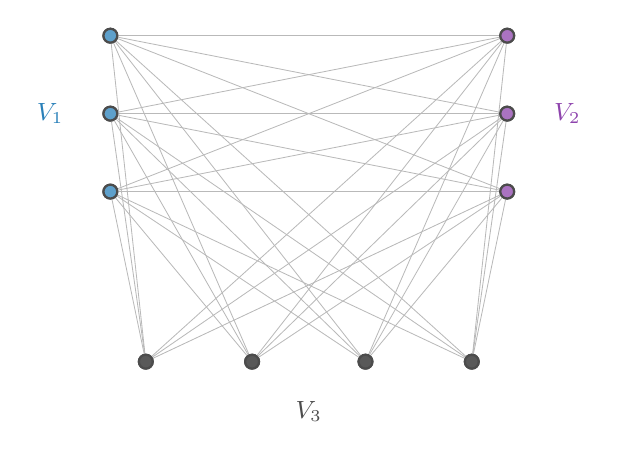
\begin{tikzpicture}[scale=0.9,
    vtx/.style={circle, draw=black!70, thick, minimum size=5pt, inner sep=0pt},
    edgestyle/.style={gray!55, line width=0.3pt}]
  \foreach \y [count=\i] in {2.2, 1.1, 0.0} {\node[vtx, fill=primary!75] (A\i) at (0,\y) {};}
  \foreach \y [count=\j] in {2.2, 1.1, 0.0} {\node[vtx, fill=secondary!75] (B\j) at (5.6,\y) {};}
  \foreach \x [count=\k] in {0.5, 2.0, 3.6, 5.1} {\node[vtx, fill=black!65] (C\k) at (\x,-2.4) {};}
  \foreach \i in {1,2,3}{\foreach \j in {1,2,3}{\draw[edgestyle] (A\i)--(B\j);}}
  \foreach \i in {1,2,3}{\foreach \k in {1,2,3,4}{\draw[edgestyle] (A\i)--(C\k);}}
  \foreach \j in {1,2,3}{\foreach \k in {1,2,3,4}{\draw[edgestyle] (B\j)--(C\k);}}
  \foreach \i in {1,2,3}{\node[vtx, fill=primary!75] at (A\i) {};}
  \foreach \j in {1,2,3}{\node[vtx, fill=secondary!75] at (B\j) {};}
  \foreach \k in {1,2,3,4}{\node[vtx, fill=black!65] at (C\k) {};}
  \node[primary, font=\small\bfseries] at (-0.85,1.1) {$V_1$};
  \node[secondary, font=\small\bfseries] at (6.45,1.1) {$V_2$};
  \node[black!70, font=\small\bfseries] at (2.8,-3.1) {$V_3$};
\end{tikzpicture}
\caption{The Tur\'an graph $T_{10,3}=K_{3,3,4}$: all edges between distinct
parts, none within a part.}
\label{fig:turangraph}
\end{figure}

\begin{theorem}{Tur\'an's theorem (weak form), 1941}{turanthm}
An $n$-vertex $K_{r+1}$-free graph has at most
$\bigl(1-\tfrac1r\bigr)\dfrac{n^2}{2}$ edges.
\end{theorem}

\begin{proof}
Let $m=|E(G)|$. As $G$ is $K_{r+1}$-free, its clique number is at most $r$, so
Corollary~\ref{cor:carowei-clique} together with the AM--HM inequality (the
convexity of $x\mapsto 1/x$ applied to the values $n-d_v$, using
$\sum_v d_v=2m$) gives
\[
  r \;\ge\; \sum_{v\in V}\frac{1}{n-d_v}
    \;\ge\; \frac{n}{\,n-\frac1n\sum_v d_v\,}
    \;=\; \frac{n}{\,n-\frac{2m}{n}\,}.
\]
Rearranging $r\bigl(n-\tfrac{2m}{n}\bigr)\ge n$ yields
$m\le\bigl(1-\tfrac1r\bigr)\tfrac{n^2}{2}$.
\end{proof}

\begin{remark}{Tightness}{turanremark}
A refinement recovers the full theorem: for fixed $\sum_v d_v$, the sum
$\sum_v 1/(n-d_v)$ is smallest when the degrees are as equal as possible,
which is exactly the structure of $T_{n,r}$. The bound is asymptotically
sharp, and its $r=2$ case is Mantel's theorem: a triangle-free graph has at
most $n^2/4$ edges.
\end{remark}

\begin{insight}
Caro--Wei is strictly stronger than the Tur\'an bound it implies: it is
degree-by-degree sensitive and exact for unions of cliques, whereas Tur\'an
sees only $n$ and $m$. The implication runs one way --- a sharp local
estimate manufactures the coarse global one --- and the convexity step is
where extremality enters, simultaneously producing the inequality and singling
out $T_{n,r}$ as the unique optimum.
\end{insight}

% =====================================================================
\section{Bounding by sampling}
% =====================================================================

The hypergraph analogue of Tur\'an's problem is far harder. A
\emph{tetrahedron} $K_4^{(3)}$ is the complete $3$-uniform hypergraph on $4$
vertices --- the four triples one can form, like the faces of a solid
tetrahedron.

\begin{question}{Hypergraph Tur\'an problem for tetrahedra}{tetraturan}
What is the maximum number of edges in an $n$-vertex $3$-uniform hypergraph
with no tetrahedron?
\end{question}

This is a famous open problem. Tur\'an conjectured the extremal density to be
$\tfrac59$, achievable by partitioning the vertices into three nearly equal
parts $V_1,V_2,V_3$ and taking all transversal triples together with all
``$2{+}1$'' triples (two vertices in $V_i$, one in $V_{i+1}$, indices mod
$3$); notably, several non-isomorphic constructions reach the same density.
Rather than chase the exact answer, we illustrate a versatile averaging idea.

\begin{proposition}{Cheap sampling bound}{sample4}
A tetrahedron-free $3$-graph on $n\ge4$ vertices has at most
$\tfrac34\binom n3$ edges.
\end{proposition}

\begin{proof}
Choose a uniformly random $4$-set $S$ of vertices. If the hypergraph has
$p\binom n3$ edges, then each triple is contained in $S$ with the same
probability, and linearity gives an expected $4p$ edges induced by $S$.
Tetrahedron-freeness means $S$ spans at most $3$ of its $4$ triples, so
$4p\le 3$, whence the edge count $p\binom n3\le\tfrac34\binom n3$.
\end{proof}

A larger sampling window does better, provided we solve the corresponding
small case.

\begin{lemma}{Five-vertex bound}{fivevertex}
A tetrahedron-free $3$-graph on $5$ vertices has at most $7$ edges.
\end{lemma}

\begin{proof}
Replace each triple by its complement to obtain an ordinary graph $G$ on the
same $5$ vertices (a triple is present in $G$'s ``co-structure'' exactly when
it is absent from the hypergraph). A tetrahedron --- four vertices spanning
all four of their triples --- corresponds to a vertex of degree $4$ in $G$.
So the hypergraph is tetrahedron-free iff $G$ has maximum degree at most $3$,
and a $5$-vertex graph with $\Delta\le 3$ has at most
$\lfloor 3\cdot5/2\rfloor=7$ edges, a value that is attainable.
\end{proof}

Re-running the sampling proof with $5$-vertex subsets and feeding in the bound
$7$ sharpens the estimate.

\begin{proposition}{Improved sampling bound}{sample5}
A tetrahedron-free $3$-graph on $n\ge4$ vertices has at most
$\tfrac{7}{10}\binom n3$ edges.
\end{proposition}

\begin{insight}
A sampling bound looks probabilistic but is really a double count: average
local density equals global density. The decisive structural fact is
\emph{monotone improvement} --- enlarging the window to $s$ vertices and
solving the $s$-vertex extremal problem can only tighten the bound, and in
principle converges to the true Tur\'an density. This is the conceptual seed
of Razborov's \emph{flag algebras}, which mechanize ``optimize over all local
densities'' as a semidefinite program and currently give the record upper
bound $\approx 0.561$. That the brute force is hopeless by hand --- the
$s$-vertex problem explodes --- is exactly the gap flag algebras fill.
\end{insight}

% =====================================================================
\section{Unbalancing lights}
% =====================================================================

Consider an $n\times n$ array of $\pm1$ values $a_{ij}$, where we are allowed
to flip the sign of any full row or column. Writing $x_i,y_j\in\{-1,1\}$ for
the flips, the quantity $\sum_{ij}a_{ij}x_iy_j$ equals the number of
$+1$ entries minus the number of $-1$ entries after flipping. Random flips
achieve nothing on average; the gain comes from mixing randomness with greed.

\begin{theorem}{}{lights}
For any $a_{ij}\in\{-1,1\}$ there exist $x_i,y_j\in\{-1,1\}$ with
\[
  \sum_{i,j=1}^n a_{ij}\,x_i\,y_j
  \;\ge\; \Bigl(\sqrt{\tfrac{2}{\pi}}+o(1)\Bigr)\,n^{3/2}.
\]
\end{theorem}

\begin{proof}
Choose the column signs $y_1,\dots,y_n\in\{-1,1\}$ independently and
uniformly. For each row $i$ set $R_i=\sum_j a_{ij}y_j$, and then choose
$x_i=\operatorname{sign}(R_i)$ (breaking ties arbitrarily). This greedy choice
maximizes each row's contribution, so
\[
  \sum_{i=1}^n R_i x_i = \sum_{i=1}^n |R_i|.
\]
For each fixed $i$, $R_i$ is distributed like a signed sum
$S_n=\varepsilon_1+\cdots+\varepsilon_n$ of $n$ i.i.d.\ uniform $\pm1$ signs
(the $R_i$ are not mutually independent, but linearity does not require it).
By the central limit theorem,
\[
  \lim_{n\to\infty}\E\!\left[\frac{|S_n|}{\sqrt n}\right]
   = \E|Z| = \frac{1}{\sqrt{2\pi}}\int_{\mathbb{R}}|x|\,e^{-x^2/2}\,dx
   = \sqrt{\tfrac{2}{\pi}}, \qquad Z\sim\mathcal N(0,1),
\]
so $\E|R_i|=(\sqrt{2/\pi}+o(1))\sqrt n$. (One can even compute exactly,
$\E|S_n|=n\,2^{1-n}\binom{n-1}{\lfloor (n-1)/2\rfloor}$, though it is not
needed.) Summing over the $n$ rows, $\E\sum_i|R_i|=(\sqrt{2/\pi}+o(1))n^{3/2}$,
and the averaging principle finishes the proof.
\end{proof}

\begin{insight}
The technique is \emph{randomize-then-optimize}: leaving the rows
deterministic and choosing them after seeing the random columns is what beats
the trivial half. The constant $\sqrt{2/\pi}=\E|\mathcal N(0,1)|$ is the
tell-tale of a Gaussian hiding in a discrete problem. Read as discrepancy,
the $n^{3/2}$ growth is $n$ rows each fluctuating on the universal
$\sqrt n$ scale --- the same square-root law behind Khintchine's inequality.
\end{insight}

The next result runs a probabilistic process whose parameters are never named;
a compactness argument supplies them.

\begin{theorem}{}{kuniform}
Let $k\ge2$ and $V=V_1\cup\cdots\cup V_k$ with the $V_i$ disjoint of size $n$.
Two-colour the edges of the complete $k$-uniform hypergraph on $V$, with every
transversal edge (one vertex per $V_i$) coloured blue. Then there is a set
$S\subseteq V$ in which the numbers of red and blue edges differ by more than
$c_k n^k$, for a constant $c_k>0$.
\end{theorem}

\begin{proof}[Proof sketch]
Write the proof for $k=3$; the general case is identical. Include each vertex
of $V_i$ independently with probability $p_i$, to be chosen. With
$a_{i,j,k}$ the blue-minus-red edge count across $V_i\times V_j\times V_k$,
the expected blue-minus-red total inside $S$ is a polynomial
\[
  f(p_1,p_2,p_3)=\sum_{i\le j\le k}a_{i,j,k}\,p_ip_jp_k,
\]
whose coefficients satisfy $|a_{i,j,k}|\le n^3$ and whose
$p_1p_2p_3$-coefficient equals $n^3$ by the transversal-blue hypothesis.
Dividing by $n^3$, it suffices to make $|f|>cn^3$ for an absolute $c>0$; this
is supplied by the next lemma applied to $f/n^3$.
\end{proof}

\begin{lemma}{Compactness lemma}{compactness}
Let $P_k$ be the set of degree-$k$ polynomials in $p_1,\dots,p_k$ whose
coefficients are bounded by $1$ in absolute value and whose
$p_1p_2\cdots p_k$-coefficient equals $1$. Then there is a constant $c_k>0$
such that every $g\in P_k$ satisfies $|g(p_1,\dots,p_k)|\ge c_k$ for some
$p_1,\dots,p_k\in[0,1]$.
\end{lemma}

\begin{proof}
Let $M(g)=\max_{[0,1]^k}|g|$; the maximum exists by compactness of the cube.
Each $g\in P_k$ is nonzero (its top coefficient is $1$), so $M(g)>0$. The set
$P_k$ is compact and $M$ is continuous, so $M$ attains a positive minimum
$c_k=\min_{g\in P_k}M(g)>0$, which works for all of $P_k$.
\end{proof}

\begin{insight}
This argument never exhibits the winning probabilities: compactness
\emph{guarantees} the constant $c_k$ exists without computing it, because the
space of normalized polynomials is compact and ``best value on the cube'' is a
continuous, strictly positive function. It is the probabilistic method in
purely existential mode --- the cost being an ineffective constant.
\end{insight}

% =====================================================================
\section{The crossing number inequality}
% =====================================================================

\begin{definition}{Crossing number}{crossingnumber}
For a drawing of a graph in the plane with edges as continuous curves, count
its edge crossings. The \emph{crossing number} $\cross(G)$ is the minimum over
all drawings. A graph is \emph{planar} when $\cross(G)=0$.
\end{definition}

The graphs $K_5$ and $K_{3,3}$ are the only obstructions to planarity:
Kuratowski's theorem (1930) characterizes planarity by the absence of a
subdivision of either, and Wagner's theorem (1937) by the absence of either as
a minor. The quantitative question is whether many edges force many crossings.

\begin{theorem}{Crossing number inequality (ACNS 1982, Leighton 1984)}{crossing}
If $|E|\ge 4|V|$, then $\displaystyle \cross(G)\gtrsim\frac{|E|^3}{|V|^2}$.
\end{theorem}

\begin{proof}
\textbf{Step 1 (zero to one).} Euler's formula $v-e+f=2$ for a connected
planar drawing, combined with $3f\le 2e$ (each face borders $\ge3$ edges, each
edge borders $2$ faces), gives $|E|\le 3|V|-6$, hence $|E|\le 3|V|$ for every
planar graph. So $|E|>3|V|$ forces at least one crossing.

\smallskip\noindent\textbf{Step 2 (one to many).} Deleting one edge per
crossing in an optimal drawing planarizes $G$, leaving
$|E|-\cross(G)\le 3|V|$ edges, i.e.\ $\cross(G)\ge|E|-3|V|$. For
$|E|=\Theta(n^2)$ this only gives $\cross(G)\gtrsim n^2$ --- weak.

\smallskip\noindent\textbf{Step 3 (bootstrapping).} Fix $p\in[0,1]$ and let
$G'$ keep each vertex independently with probability $p$. Apply Step~2 to
$G'$ and take expectations. A crossing survives iff all four endpoints are
kept, so $\E\,\cross(G')\le p^4\cross(G)$; an edge survives iff both endpoints
are kept, so $\E|E'|=p^2|E|$; and $\E|V'|=p|V|$. Thus
\[
  p^4\cross(G)\ge p^2|E|-3p|V|,\qquad\text{so}\qquad
  \cross(G)\ge p^{-2}|E|-3p^{-3}|V|.
\]
Choosing $p=4|V|/|E|\in[0,1]$ (valid since $|E|\ge4|V|$) balances the two
terms and gives $\cross(G)\gtrsim|E|^3/|V|^2$.
\end{proof}

\begin{corollary}{}{crossingcor}
If $|E|\gtrsim|V|^2$, then $\cross(G)\gtrsim|V|^4$.
\end{corollary}

\begin{insight}
Step~3 is pure amplification: a deterministic bound that is laughable on dense
graphs becomes sharp once applied to a randomly thinned copy and rescaled,
because crossings, edges, and vertices scale as $p^4,p^2,p^1$ and tuning $p$
exploits the gap. Two caveats. Sampling \emph{vertices} is essential ---
sampling edges fails, since the cheap bound is anchored to the vertex count.
And the inequality's fame rests on an application not stated here: it yields a
one-line proof of the Szemer\'edi--Trotter point--line incidence bound
$I(P,L)\lesssim(|P||L|)^{2/3}+|P|+|L|$, turning an extremal-graph estimate into
a cornerstone of combinatorial geometry.
\end{insight}

% =====================================================================
\section*{Exercises}
\addcontentsline{toc}{section}{Exercises}
% =====================================================================

\begin{enumerate}[itemsep=4pt]
  \item Let $A$ be a measurable subset of the unit sphere in $\mathbb{R}^3$
        containing no pair of orthogonal points.
        \begin{enumerate}
          \item Prove that $A$ occupies at most $1/3$ of the sphere's area.
          \item $\bigstar$ Prove an upper bound strictly smaller than $1/3$.
        \end{enumerate}
  \item $\bigstar$ Prove that every set of $10$ points in the plane can be
        covered by a union of disjoint unit disks.
  \item Let $\mathbf r=(r_1,\dots,r_k)$ be nonzero integers with nonzero sum.
        Prove there is a constant $c>0$ (depending only on $\mathbf r$) such
        that every finite set $A$ of nonzero reals has a subset $B\subseteq A$
        with $|B|\ge c|A|$ admitting no $b_1,\dots,b_k\in B$ with
        $r_1b_1+\cdots+r_kb_k=0$.
  \item Prove that every set $A$ of $n$ nonzero integers contains two disjoint
        sum-free subsets $B_1,B_2$ with $|B_1|+|B_2|>2n/3$.
  \item Let $G$ be an $n$-vertex graph with $pn^2$ edges, $n\ge10$ and
        $p\ge10/n$. Prove $G$ contains a pair of vertex-disjoint, isomorphic
        subgraphs, each with at least $c\,p^2n^2$ edges for some constant
        $c>0$.
  \item $\bigstar$ Prove that for every $r$ there is an integer $K$ such that
        the following holds: if $S$ is a set of $rk$ evenly spaced points on a
        circle, partitioned as $S=S_1\cup\cdots\cup S_r$ with $|S_i|=k$, then
        for $k\ge K$ there exist $r$ congruent triangles, the $i$-th with all
        vertices in $S_i$.
  \item $\bigstar$ Prove that $[n]^d$ cannot be partitioned into fewer than
        $2^d$ sets, each of the form $A_1\times\cdots\times A_d$ with
        $A_i\subsetneq[n]$.
\end{enumerate}

% =====================================================================
%  Chapter 3 — Alterations
%  File: chapters/03_alterations.tex
%  Styled to match Chapters 1-2 (boxed environments + Insight callouts).
%  Cross-references Chapter 1 (alteration, 2-colourability baseline) and
%  Appendix A (Markov) instead of repeating them.
% =====================================================================
\providecommand{\E}{\mathbb{E}}
\providecommand{\Prob}{\mathbb{P}}
\providecommand{\ind}{\mathbf{1}}

\chapter{Alterations}
\label{chap:alterations}

The first moment, used bare, asks a random object to be perfect. The
\emph{alteration method} asks only that it be \emph{nearly} perfect, then pays
to repair the few defects. We met it briefly in Chapter~1, where a random
$2$-colouring of $K_n$ was patched into a Ramsey colouring by deleting one
vertex from each monochromatic clique (Theorem~\ref{thm:ramsey_alt}). The
accounting is always the same: bound the expected number of blemishes by the
first moment, subtract it from what you started with, and conclude that some
outcome leaves enough behind. This chapter pushes the idea through four
problems of increasing subtlety --- dominating sets, the Heilbronn triangle
problem, graphs of high girth and high chromatic number, and the best known
bound for two-colourable hypergraphs.

\begin{insight}
The reason alteration so often beats the bare first moment is a division of
labour. A single random construction must simultaneously be large \emph{and}
defect-free, and demanding both at once is wasteful. Alteration decouples them:
make the object as large as you like and tolerate defects, then spend a
controlled amount of that size erasing them. The net size is
(initial size) $-$ (expected repairs), and as long as the repairs are a lower-order
cost, you keep almost everything. Watch for this two-line structure --- build
generously, then delete --- in every proof below.
\end{insight}

% =====================================================================
\section{Dominating sets}
% =====================================================================

\begin{definition}{Dominating set}{dominating}
In a graph $G=(V,E)$, a set $U\subseteq V$ is \emph{dominating} if every vertex
outside $U$ has a neighbour inside $U$.
\end{definition}

\begin{theorem}{Small dominating sets}{dominating-thm}
Every $n$-vertex graph with minimum degree $\delta\ge1$ has a dominating set of
size at most
\[
  \frac{1+\log(\delta+1)}{\delta+1}\;n.
\]
\end{theorem}

\begin{proof}
Fix $p\in[0,1]$, to be chosen. Include each vertex in a random set $X$
independently with probability $p$, and let
\[
  Y = V\setminus\bigl(X\cup N(X)\bigr)
\]
be the vertices that are neither chosen nor adjacent to a chosen vertex. Then
$X\cup Y$ is dominating: any vertex outside it lies in $X\cup N(X)$, hence has a
neighbour in $X$.

A vertex $v$ lands in $Y$ only if $v$ and all of its $\deg(v)\ge\delta$
neighbours avoid $X$ --- that is $1+\deg(v)\ge1+\delta$ independent misses --- so
$\Prob(v\in Y)\le(1-p)^{1+\delta}$. By linearity,
\[
  \E|X\cup Y| = \E|X|+\E|Y|
  \le pn + (1-p)^{1+\delta}n
  \le \bigl(p + e^{-p(1+\delta)}\bigr)n,
\]
using $1-p\le e^{-p}$. The bracket is minimized at
$p=\dfrac{\log(\delta+1)}{\delta+1}$, where $e^{-p(\delta+1)}=\dfrac{1}{\delta+1}$,
giving the value $\dfrac{1+\log(\delta+1)}{\delta+1}$. Some outcome attains at
most the expectation.
\end{proof}

\begin{insight}
The trivial lower bound on a dominating set is $n/(\delta+1)$ --- each chosen
vertex can cover at most $\delta+1$ vertices --- and this theorem says you can
come within a $\log(\delta+1)$ factor of it. A greedy algorithm (repeatedly
take the vertex covering the most as-yet-uncovered vertices) achieves the same
order and is in fact the standard \textsc{Set-Cover} greedy, whose
$\log$ factor is known to be unavoidable in general. What the alteration proof
buys is brevity: the messy, history-dependent greedy analysis is replaced by a
one-line expectation, with the optimal $p$ falling out of a single derivative.
\end{insight}

% =====================================================================
\section{The Heilbronn triangle problem}
% =====================================================================

\begin{question}{Heilbronn's problem}{heilbronn-q}
How should one place $n$ points in the unit square so that the smallest triangle
they span is as large as possible? Writing
\[
  \Delta(n) = \sup_{\substack{S\subseteq[0,1]^2\\|S|=n}}\
  \min_{\substack{p,q,r\in S\\\text{distinct}}} \operatorname{area}(pqr),
\]
how does $\Delta(n)$ behave?
\end{question}

Naive placements do poorly. Points equally spaced on a circle leave a triangle
of area $\Theta(n^{-3})$ (three consecutive points), and a grid does worse
still --- three collinear points give area zero. Heilbronn conjectured
$\Delta(n)=O(n^{-2})$; Koml\'os, Pintz, and Szemer\'edi (1982) disproved it,
showing $\Delta(n)\gtrsim n^{-2}\log n$ by an intricate random construction.
Here is a simpler argument for the weaker --- but already conjecture-refuting in
spirit --- bound $\Delta(n)\gtrsim n^{-2}$.

\begin{theorem}{Many points, no small triangle}{heilbronn-thm}
For every $n$ there is a set of $n$ points in $[0,1]^2$ in which every triple
spans a triangle of area at least $cn^{-2}$, for an absolute constant $c>0$.
\end{theorem}

\begin{proof}
Scatter $2n$ points independently and uniformly in $[0,1]^2$, and estimate the
chance that a fixed triple is nearly collinear. The distance between two random
points satisfies, by an annulus area estimate,
$\Prob(|pq|\in[x,x+dx])\le 2\pi x\,dx$. Conditioning on $p,q$, the triangle
$pqr$ has area at most $\varepsilon$ exactly when $r$ lies within distance
$2\varepsilon/|pq|$ of the line through $p,q$, a strip of area
$\lesssim \varepsilon/|pq|$ inside the square. Hence
\[
  \Prob\bigl(\operatorname{area}(pqr)\le\varepsilon\bigr)
  \;\lesssim\;\int_0^{\sqrt2} 2\pi x\cdot\frac{\varepsilon}{x}\,dx
  \;\asymp\;\varepsilon.
\]
Let $X$ count the triples of area at most $\varepsilon$. There are
$\binom{2n}{3}=O(n^3)$ triples, so $\E[X]=O(\varepsilon n^3)$. Choosing
$\varepsilon=c/n^2$ with $c$ small makes $\E[X]\le n$.

Now \emph{alter}: delete one point from each offending triple. At least
$2n-X$ points survive, with expectation $\E[2n-X]\ge n$, and the survivors
contain no triangle of area below $\varepsilon=c/n^2$. Some outcome therefore
leaves $\ge n$ points with every triangle of area $\ge cn^{-2}$.
\end{proof}

\begin{remark}{An explicit construction}{heilbronn-algebraic}
A clean derandomization, due to Erd\H{o}s, matches $\Delta(n)\gtrsim n^{-2}$
algebraically. For a prime $p$, the parabola points
$\{(x,x^2)\bmod p : x\in\mathbb F_p\}$ contain no three collinear points (a
parabola meets a line in at most two points), so viewed in the integer grid
$[p]^2$, every triangle has area at least $1/2$ by Pick's theorem. Rescaling
into the unit square gives $p$ points with all triangle areas
$\gtrsim p^{-2}$; for general $n$, use a prime between $n$ and $2n$.
\end{remark}

\begin{insight}
The probabilistic proof and the algebraic one make an instructive pair: the
random construction is effortless to set up but yields an object one cannot
write down, while the parabola is fully explicit yet requires the clever
observation that ``no three collinear'' forces area $\ge1/2$ over the integers.
The $\log n$ that Koml\'os--Pintz--Szemer\'edi gained over both comes from a far
more careful random construction in which the deletions are correlated rather
than treated independently --- a recurring theme: the easy alteration leaves a
logarithmic factor on the table.
\end{insight}

% =====================================================================
\section{Markov's inequality, recalled}
% =====================================================================

The next two sections lean on a single tail bound, proved in
Appendix~\ref{chap:toolkit}: for a nonnegative random variable $X$ and any
$a>0$,
\[
  \Prob(X\ge a)\le\frac{\E[X]}{a}.
\]
In words --- if $\E[X]$ is small, then $X$ is small typically, not merely on
average. This is what lets the alteration method control not just the expected
number of defects but the probability of having too many at once.

% =====================================================================
\section{High girth and high chromatic number}
% =====================================================================

A $k$-clique forces chromatic number at least $k$, a lower bound certified by
purely local information. Is high chromatic number \emph{always} locally
certifiable? The following construction says emphatically no: a graph can be
locally indistinguishable from a tree --- no short cycles at all --- and still
require many colours.

\begin{definition}{Girth}{girth}
The \emph{girth} of a graph is the length of its shortest cycle (infinite if the
graph is a forest).
\end{definition}

\begin{theorem}{Erd\H{o}s 1959}{girth-chromatic}
For every $k$ and $\ell$, there is a graph with girth greater than $\ell$ and
chromatic number greater than $k$.
\end{theorem}

\begin{proof}
Take the Erd\H{o}s--R\'enyi random graph $G\sim G(n,p)$ on $n$ vertices, each
edge present independently with probability $p=(\log n)^2/n$. We control two
features and then delete.

\smallskip\noindent\emph{Short cycles.} Let $X$ count the cycles of length at
most $\ell$. Since $K_n$ has $\binom ni(i-1)!/2\le n^i$ cycles of length $i$,
linearity gives
\[
  \E[X]=\sum_{i=3}^{\ell}\binom ni\frac{(i-1)!}{2}\,p^i
  \le\sum_{i=3}^{\ell}(np)^i
  =\sum_{i=3}^{\ell}(\log n)^{2i}=o(n),
\]
as $\ell$ is constant. By Markov, $\Prob(X\ge n/2)\le \E[X]/(n/2)=o(1)$.

\smallskip\noindent\emph{Large independent sets.} Recall
$\chi(G)\ge |V(G)|/\alpha(G)$, where $\alpha$ is the independence number, so it
suffices to keep $\alpha$ small. With $x=\lceil 3n/\log n\rceil=(3/p)\log n$,
\[
  \Prob\bigl(\alpha(G)\ge x\bigr)\le\binom nx(1-p)^{\binom x2}
  < n^x e^{-p x(x-1)/2}
  = \bigl(n\,e^{-p(x-1)/2}\bigr)^x = o(1),
\]
because $p(x-1)/2\sim\tfrac32\log n$ makes the base $n\cdot n^{-3/2}=n^{-1/2}$.

\smallskip\noindent\emph{Alteration.} For $n$ large, both bad events have
probability below $1/2$, so some $G$ has fewer than $n/2$ short cycles and
$\alpha(G)\le 3n/\log n$. Delete one vertex from each cycle of length
$\le\ell$ to obtain $G'$. Then $|V(G')|\ge n/2$, the girth exceeds $\ell$,
$\alpha(G')\le\alpha(G)\le 3n/\log n$, and
\[
  \chi(G')\ge\frac{|V(G')|}{\alpha(G')}\ge\frac{n/2}{3n/\log n}
  =\frac{\log n}{6}>k
\]
once $n$ is large enough.
\end{proof}

\begin{insight}
This is the alteration method at full power, and the choice $p=(\log n)^2/n$ is
delicate: $p$ must be small enough that short cycles are rare
($np$ only polylogarithmic) yet large enough that independent sets are tiny.
The conclusion is conceptually startling --- high chromatic number is a
\emph{global} property, invisible to any bounded neighbourhood, since a girth
exceeding $\ell$ means every ball of radius $\ell/2$ is a tree. Erd\H{o}s (1962)
sharpened this: there are graphs of chromatic number $>k$ in which \emph{every}
linear-sized subgraph is $3$-colourable, so even seeing a constant fraction of
the graph need not reveal its true colourability.
\end{insight}

% =====================================================================
\section{Random greedy colouring}
% =====================================================================

In Chapter~1 we showed (Theorem~\ref{thm:hyper_lower}) that any $k$-uniform
hypergraph with fewer than $2^{k-1}$ edges is $2$-colourable. We now improve the
threshold by a factor of order $\sqrt{k/\log k}$, via a random greedy colouring.

\begin{theorem}{Radhakrishnan--Srinivasan 2000}{greedy-colouring}
There is a constant $c>0$ such that every $k$-uniform hypergraph with at most
$c\sqrt{\dfrac{k}{\log k}}\;2^{k}$ edges is $2$-colourable.
\end{theorem}

\begin{proof}
Order the vertices by a uniformly random permutation and colour greedily from
left to right: make each vertex blue unless doing so would complete an
all-blue edge, in which case make it red. By construction no edge is all blue,
so the colouring fails only if some edge ends up all red.

\smallskip\noindent\emph{Conflicting pairs.} If a red edge appears, its last
vertex $v$ was forced red, meaning $v$ already completed an all-blue edge $e$
(so $v$ is the \emph{last} vertex of $e$) while also being the \emph{first}
vertex of the red edge $f$. Thus there are two edges $e,f$ sharing the single
vertex $v$, with $v$ last in $e$ and first in $f$; call such an ordered pair
\emph{conflicting}. Crucially, whether $(e,f)$ conflicts depends only on the
random ordering, not on the colours. For two edges meeting in exactly one
vertex (so $2k-1$ vertices in all), conflict requires $v$ to follow the other
$k-1$ vertices of $e$ and precede the other $k-1$ of $f$:
\[
  \Prob\bigl((e,f)\text{ conflicts}\bigr)=\frac{(k-1)!^2}{(2k-1)!}
  \asymp k^{-1/2}2^{-2k}.
\]
Summing over the at most $m^2$ such ordered pairs, the expected number of
conflicting pairs is $\lesssim m^2 k^{-1/2}2^{-2k}$, which is below $1$ once
$m\asymp k^{1/4}2^k$. This already gives a bound (Pluh\'ar 2009); we now sharpen
it.

\smallskip\noindent\emph{The $L\cup M\cup R$ refinement.} Instead of a bare
permutation, drop each vertex at an independent uniform position in $[0,1]$, and
split the interval (with $p$ to be chosen) into
\[
  L=\Bigl[0,\tfrac{1-p}2\Bigr),\quad
  M=\Bigl[\tfrac{1-p}2,\tfrac{1+p}2\Bigr],\quad
  R=\Bigl(\tfrac{1+p}2,1\Bigr].
\]
A fixed edge lands entirely in $L$ with probability $(\tfrac{1-p}2)^k$, and
likewise for $R$, so
\[
  \Prob(\text{some edge lies in }L\text{ or }R)\le 2m\Bigl(\tfrac{1-p}2\Bigr)^k.
\]
Suppose no edge lies wholly in $L$ or $R$. If $(e,f)$ conflicts with shared
vertex $v$, then every vertex of $e$ precedes $v$ and every vertex of $f$
follows it; were $v\in L$ then $e\subseteq L$, and were $v\in R$ then
$f\subseteq R$ --- both excluded. So $v\in M$, and
\[
  \Prob\bigl((e,f)\text{ conflicts, }v\in M\bigr)
  =\int_{(1-p)/2}^{(1+p)/2}x^{k-1}(1-x)^{k-1}\,dx
  \le p\,4^{-k+1},
\]
using $x(1-x)\le\tfrac14$. Union-bounding over $\le m^2$ pairs and combining,
\[
  \Prob(\text{some conflict})
  \le 2m\Bigl(\tfrac{1-p}2\Bigr)^k + m^2 p\,4^{-k+1}
  < 2^{-k+1}m\,e^{-pk} + \bigl(2^{-k+1}m\bigr)^2 p.
\]
Setting $p=\dfrac{1}{k}\log\!\dfrac{2^{k-1}k}{m}$ to minimize the right-hand
side makes it
\[
  \frac{m^2}{4^{k-1}k}\Bigl(1+\log\tfrac{2^{k-1}k}{m}\Bigr),
\]
which is $<1$ when $m=c\,2^k\sqrt{k/\log k}$ for a small constant $c>0$ (taking
$k$ large enough that $p\in[0,1]$; small $k$ are absorbed by shrinking $c$).
With positive probability there is then no conflicting pair, so the greedy
colouring produces no red edge and succeeds.
\end{proof}

\begin{insight}
Where did the improvement come from? The expected number of conflicting pairs
is essentially unchanged --- the $L\cup M\cup R$ device does not make conflicts
rarer on average. What it does is \emph{cluster} the bad events. By first paying
a cheap union bound to forbid any edge from sitting in an extreme block, the
remaining conflicts are confined to a shared common vertex in the thin middle
strip $M$, and the second-order term picks up a factor $p$ (the width of $M$)
that a naive count would miss. Exploiting positive correlation among bad events
that share a localized cause --- rather than bounding them as if independent ---
is the engine of the gain, and squeezing more out of this idea remains an
intriguing open problem.
\end{insight}

% =====================================================================
\section*{Exercises}
\addcontentsline{toc}{section}{Exercises}
% =====================================================================

\begin{enumerate}[itemsep=4pt]
  \item Using the alteration method, prove the Ramsey bound
        $R(4,k)\ge c\,(k/\log k)^2$ for some constant $c>0$.
  \item Prove that every $3$-uniform hypergraph with $n$ vertices and $m\ge n$
        edges contains an independent set (a vertex set spanning no edge) of size
        at least $c\,n^{3/2}/\sqrt m$, for a constant $c>0$.
  \item Prove that every $k$-uniform hypergraph with $n$ vertices and $m$ edges
        has a transversal (a vertex set meeting every edge) of size at most
        $n(\log k)/k+m/k$.
  \item (Zarankiewicz.) Prove that for all $n\ge k\ge2$ there is an $n\times n$
        $\{0,1\}$-matrix with at least $\tfrac12 n^{2-2/(k+1)}$ ones containing no
        all-ones $k\times k$ submatrix.
  \item Fix $k$. Prove there is a constant $c_k>1$ so that for all large $n$
        there exist at least $c_k^{\,n}$ subsets of $[n]$ such that for every $k$
        distinct members $F_1,\dots,F_k$, all $2^k$ intersections
        $\bigcap_i G_i$ are nonempty, where each $G_i$ is $F_i$ or its complement.
  \item (Acute sets.) Prove that for some $c>0$ and every $n$ there are at least
        $c\,(2/\sqrt3)^n$ subsets of $[n]$ with no three distinct members
        $A,B,C$ satisfying $A\cap B\subseteq C\subseteq A\cup B$; deduce a set of
        $\ge c\,(2/\sqrt3)^n$ points in $\mathbb R^n$ spanning only acute angles.
  \item $\bigstar$ Covering complements of sparse graphs by cliques.
        \begin{enumerate}
          \item Prove every $n$-vertex graph with minimum degree $n-d$ is a union
                of $O(d^2\log n)$ cliques.
          \item Prove every bipartite graph with $n$ vertices per side and minimum
                degree $n-d$ ($d\ge1$) is a union of $O(d\log n)$ complete
                bipartite graphs.
        \end{enumerate}
  \item $\bigstar$ Let $G$ have $n$ vertices and minimum degree $\delta\ge2$.
        Prove there is $A\subseteq V$ with $|A|=O(n(\log\delta)/\delta)$ such that
        every vertex outside $A$ has a neighbour in $A$ \emph{and} a neighbour
        outside $A$.
  \item $\bigstar$ Prove every graph $G$ without isolated vertices has an induced
        subgraph on at least $\alpha(G)/2$ vertices in which every vertex has odd
        degree.
\end{enumerate}

% =====================================================================
%  Chapter 4 — The Second Moment Method
%  File: chapters/04_second_moment.tex
% =====================================================================
\providecommand{\E}{\mathbb{E}}
\providecommand{\Prob}{\mathbb{P}}
\providecommand{\Var}{\operatorname{Var}}
\providecommand{\Cov}{\operatorname{Cov}}
\providecommand{\whp}{\textit{whp}}

\chapter{The Second Moment Method}
\label{chap:second-moment}

The first moment gives the mean of a random variable but nothing about its
spread. The \emph{second moment method} adds that control: if the variance of
$X$ is small next to $\E[X]^2$, then $X$ rarely strays far from its mean, and in
particular is usually positive. Throughout, \whp\ (``with high probability'')
means with probability tending to $1$ as $n\to\infty$.

\begin{proposition}{The second-moment criterion}{criterion}
For a nonnegative random variable $X$ with $\E[X]>0$,
\[
  \Prob(X=0)\le\frac{\Var(X)}{\E[X]^2}.
\]
Consequently, if $\E[X]>0$ and $\Var(X)=o\bigl(\E[X]^2\bigr)$ along a sequence,
then $X>0$ \whp.
\end{proposition}

\begin{proof}
If $X=0$ then $|X-\E X|=\E X$, so $\{X=0\}\subseteq\{|X-\E X|\ge\E X\}$, and
Chebyshev's inequality (Appendix~\ref{chap:toolkit}, Theorem~\ref{thm:chebyshev})
bounds the latter by $\Var(X)/\E[X]^2$.
\end{proof}

\begin{insight}
A second-moment proof is really a claim that the summands are nearly
uncorrelated. The mean $\E[X]=\sum_i\E[X_i]$ ignores dependence; the variance
$\Var(X)=\sum_i\Var(X_i)+\sum_{i\ne j}\Cov(X_i,X_j)$ measures it. So the work is
always to check that the covariance sum is small next to $\E[X]^2$. When it is,
we can pass from ``$\E[X]>0$'' to ``$X>0$ \whp'', which is what locating a
threshold requires.
\end{insight}

% =====================================================================
\section{Does a random graph contain a triangle?}
% =====================================================================

The \emph{Erd\H{o}s--R\'enyi random graph} $G(n,p)$ has $n$ vertices, each of the
$\binom n2$ edges present independently with probability $p$ (Appendix~\ref{chap:toolkit}).

\begin{question}{Triangle threshold}{triangle-q}
For which $p=p(n)$ does $G(n,p)$ contain a triangle \whp?
\end{question}

Let $X$ count the triangles. There are $\binom n3$ candidate triples, each a
triangle with probability $p^3$, so $\E[X]=\binom n3 p^3\asymp (np)^3$. This
suggests the transition happens near $p\asymp 1/n$, and the two moments confirm
it from opposite sides.

\begin{theorem}{Triangle threshold}{triangle-threshold}
If $np\to0$ then $G(n,p)$ is triangle-free \whp; if $np\to\infty$ then $G(n,p)$
contains a triangle \whp. Thus $p=1/n$ is a threshold.
\end{theorem}

\begin{proof}
If $np\to0$ then $\E[X]\asymp(np)^3\to0$, and Markov gives
$\Prob(X\ge1)\le\E[X]\to0$: no triangle \whp.

If $np\to\infty$ we use the second moment. Write $X=\sum_S\ind_S$ over triples
$S$. Two triangle-indicators are dependent only when their triples share an
edge, i.e.\ share two vertices. Grouping the covariance sum by overlap, the
only nonzero contributions come from pairs sharing exactly one edge (four
vertices, five edges), of which there are $\Theta(n^4)$, each contributing
$\Theta(p^5)$. Hence
\[
  \Var(X)\;\lesssim\;\E[X] + n^4 p^5\;\asymp\;n^3p^3+n^4p^5,
\]
while $\E[X]^2\asymp n^6p^6$. Therefore
\[
  \frac{\Var(X)}{\E[X]^2}\;\lesssim\;\frac{1}{(np)^3}+\frac{1}{n^2p}
  \;=\;\frac1{(np)^3}+\frac1{n\cdot(np)}\;\to\;0,
\]
so $X>0$ \whp\ by Proposition~\ref{prop:criterion}.
\end{proof}

\begin{insight}
The two moments split the work at the threshold. Below it $\E[X]\to0$, so Markov
alone kills the triangles. Above it $\E[X]\to\infty$ only says triangles are
expected on average; the variance bound is what rules out their all appearing
together on a rare event, and it is small here precisely because two random
triangles seldom share an edge. Right at $np\to c$ neither moment decides the
question, and the triangle count converges to a Poisson limit --- the threshold
is coarse, turning on over a constant factor rather than sharply.
\end{insight}

% =====================================================================
\section{Thresholds for fixed subgraphs}
% =====================================================================

The triangle argument generalizes to any fixed graph $H$, but with a twist: the
threshold is governed not by $H$ itself but by its densest subgraph.

\begin{definition}{Edge density and $m(H)$}{density}
The \emph{edge--vertex ratio} of a graph $H$ is $\rho(H)=e_H/v_H$ (half the
average degree), and
\[
  m(H)=\max_{H'\subseteq H}\rho(H').
\]
\end{definition}

The proof uses a packaged form of the second-moment estimate.

\begin{lemma}{Second-moment criterion via overlaps}{delta}
Let $X=\sum_i\ind_{A_i}$ with $i\sim j$ meaning $A_i,A_j$ are dependent, and set
$\Delta^\ast=\max_i\sum_{j\sim i}\Prob(A_j\mid A_i)$. If $\E[X]\to\infty$ and
$\Delta^\ast=o(\E[X])$, then $X>0$ \whp.
\end{lemma}

\begin{proof}
Since $\Var(X)\le\E[X]+\sum_i\Prob(A_i)\sum_{j\sim i}\Prob(A_j\mid A_i)
\le\E[X]\,(1+\Delta^\ast)$, Proposition~\ref{prop:criterion} gives
$\Prob(X=0)\le(1+\Delta^\ast)/\E[X]\to0$.
\end{proof}

\begin{theorem}{Subgraph threshold; Bollob\'as 1981}{subgraph-threshold}
For any fixed graph $H$, the function $p=n^{-1/m(H)}$ is a threshold for $G(n,p)$
to contain a copy of $H$.
\end{theorem}

\begin{proof}[Proof sketch]
Let $H'\subseteq H$ attain $\rho(H')=m(H)$. Below the threshold,
$\E[X_{H'}]\asymp n^{v_{H'}}p^{e_{H'}}=o(1)$, so $G(n,p)$ has no copy of $H'$,
hence none of $H$. Above the threshold, $\E[X_H]\to\infty$, and one checks
$\Delta^\ast=o(\E[X_H])$: the dominant overlaps between two copies of $H$
occur along a common subgraph $J$, and the condition $p\gg n^{-1/m(H)}\ge
n^{-1/\rho(J)}$ makes every such overlap term negligible against $\E[X_H]$.
Lemma~\ref{lem:delta} finishes the proof.
\end{proof}

\begin{insight}
A random graph gets $H$ as soon as it gets $H$'s densest subgraph; a sparse
piece hanging off a dense core shows up earlier and plays no role. That is why
the threshold is $n^{-1/m(H)}$ rather than $n^{-1/\rho(H)}$: for a pendant edge
on $K_4$ one has $\rho=7/5$ but $m=\rho(K_4)=3/2$, and it is the $K_4$ the graph
waits for.
\end{insight}

% =====================================================================
\section{The existence of thresholds}
% =====================================================================

Both examples above have a threshold. Is this a coincidence? For \emph{monotone}
properties it never is.

\begin{definition}{Threshold}{threshold}
A property $\mathcal P$ of $G(n,p)$ is \emph{increasing} if adding edges preserves
it. A sequence $r_n$ is a \emph{threshold} for $\mathcal P$ if $\Prob(G(n,p)\in
\mathcal P)\to0$ when $p/r_n\to0$ and $\to1$ when $p/r_n\to\infty$.
\end{definition}

\begin{theorem}{Bollob\'as--Thomason 1987}{threshold-exists}
Every nontrivial increasing property has a threshold.
\end{theorem}

\begin{proof}[Proof idea]
Monotonicity makes $p\mapsto\Prob(G(n,p)\in\mathcal P)$ strictly increasing, so a
\emph{critical} probability $p_c$ with $\Prob(G(n,p_c)\in\mathcal P)=1/2$ is
well defined. A \emph{multiple-exposure} argument --- running $m$ independent
copies of $G(n,p_c)$ and taking their union, which stochastically dominates
$G(n,mp_c)$ --- shows the probability jumps from near $0$ to near $1$ as $p$ moves
from $p_c/m$ to $mp_c$. Hence $p_c$ itself is a threshold.
\end{proof}

\begin{insight}
The theorem gives a threshold but not its width. Some properties ---
connectivity, or containing a fixed subgraph --- are sharp, with a transition
window narrower than the threshold; others, like containing a triangle at
$p=c/n$, are coarse, spread over a constant factor. Telling the two apart is
what the Friedgut--Bourgain theory of sharp thresholds is about.
\end{insight}

% =====================================================================
\section{The clique number of \texorpdfstring{$G(n,1/2)$}{G(n,1/2)}}
% =====================================================================

Let $\omega(G)$ be the clique number. For $G(n,1/2)$ the second moment pins it
down to two values. Write $f(n,k)=\binom nk 2^{-\binom k2}$, the expected number
of $k$-cliques.

\begin{theorem}{Second-moment bound for the clique number}{clique-sm}
If $f(n,k)\to0$ then $\omega(G(n,1/2))<k$ \whp; if $f(n,k)\to\infty$ then
$\omega(G(n,1/2))\ge k$ \whp.
\end{theorem}

\begin{proof}[Proof sketch]
The first claim is Markov: $\Prob(\omega\ge k)\le\E[X]=f(n,k)\to0$, where $X$
counts $k$-cliques. For the second, apply Lemma~\ref{lem:delta}: two $k$-sets
$S,T$ are dependent only if $|S\cap T|\ge2$, and summing
$\Prob(A_T\mid A_S)=2^{\binom{|S\cap T|}2-\binom k2}$ over such $T$ gives
$\Delta^\ast\ll\E[X]$ when $f(n,k)\to\infty$.
\end{proof}

\begin{theorem}{Two-point concentration; Bollob\'as--Erd\H{o}s, Matula 1976}{clique-2pt}
There is $k=k(n)\sim 2\log_2 n$ with
$\omega(G(n,1/2))\in\{k,k+1\}$ \whp.
\end{theorem}

\begin{proof}
The ratio of consecutive expectations is
\[
  \frac{f(n,k+1)}{f(n,k)}=\frac{n-k}{k+1}\,2^{-k}=n^{-1+o(1)}
  \qquad(k\sim2\log_2 n),
\]
so $f(n,k)$ plunges through every fixed level in a single step of $k$. Choose
$k_0\sim2\log_2 n$ with $f(n,k_0)\ge n^{-1/2}>f(n,k_0+1)$. Then
$f(n,k_0-1)\to\infty$ and $f(n,k_0+1)\to0$, so by Theorem~\ref{thm:clique-sm}
the clique number is confined to $\{k_0-1,k_0\}$ \whp.
\end{proof}

\begin{insight}
Two-point concentration is a strong conclusion: an optimization over
exponentially many subsets lands on one of two consecutive integers near
$2\log_2 n$. It works because $f(n,k)$ falls by a factor of about $n$ each time
$k$ grows by one, so there is no room in between. The same sharpness makes
$G(n,1/2)$ a convenient source of extremal objects --- its clique and independence
numbers are both $\sim2\log_2 n$ almost surely --- and Chapter~5 uses the
independence number to break the Haj\'os conjecture.
\end{insight}

% =====================================================================
\section{Hardy--Ramanujan and Erd\H{o}s--Kac}
% =====================================================================

The second moment reaches beyond graphs. Let $\nu(m)$ be the number of distinct
prime divisors of $m$.

\begin{theorem}{Hardy--Ramanujan 1917}{hardy-ramanujan}
For all but $o(n)$ of the integers $m\le n$, $\;\nu(m)=(1+o(1))\log\log n$.
\end{theorem}

\begin{proof}[Tur\'an's second-moment proof]
Pick $m$ uniformly from $[n]$ and write $\nu(m)\approx\sum_{p\le n}X_p$ where
$X_p=\ind_{p\mid m}$. Then $\E[X_p]=\lfloor n/p\rfloor/n\approx1/p$, so by
Mertens' theorem $\E[\nu]\approx\sum_{p\le n}1/p\approx\log\log n$. The pairs
$X_p,X_q$ are nearly uncorrelated ($\E[X_pX_q]\approx1/(pq)$ up to negligible
error), so $\Var(\nu)\approx\sum_p\tfrac1p(1-\tfrac1p)\approx\log\log n$ as well.
Chebyshev then gives $\nu(m)=(1+o(1))\log\log n$ outside an $o(n)$-sized
exceptional set.
\end{proof}

\begin{insight}
The heuristic is that ``divisible by $p$'' behaves like an independent coin of
bias $1/p$ across the primes. The second moment makes this precise enough to get
concentration; the method of moments pushes it to a central limit theorem
(Erd\H{o}s--Kac): $\bigl(\nu(m)-\log\log n\bigr)/\sqrt{\log\log n}$ tends to a
standard normal as $m$ ranges over $[n]$. That result is where probabilistic
number theory began.
\end{insight}

% =====================================================================
\section{Sets with distinct subset sums}
% =====================================================================

\begin{question}{Distinct sums}{distinct-q}
How small can the largest element of a set of $n$ positive integers be, if all
$2^n$ subset sums are distinct? (Powers of two give largest element $2^{n-1}$;
can one do better?)
\end{question}

\begin{theorem}{Erd\H{o}s's lower bound}{distinct-sums}
If $a_1<\cdots<a_n$ are positive integers with distinct subset sums, then
$a_n\ge c\,2^n/\sqrt n$ for an absolute constant $c>0$.
\end{theorem}

\begin{proof}
Let $\varepsilon_1,\dots,\varepsilon_n$ be independent uniform signs and put
$X=\sum_i\varepsilon_i a_i$. Then $\E[X]=0$ and
$\Var(X)=\sum_i a_i^2\le n\,a_n^2$. By Chebyshev, at least $\tfrac34$ of the
$2^n$ sign patterns yield $|X|\le 2\sqrt{\Var(X)}\le 2\sqrt n\,a_n$, i.e.\ lie
in an interval of length $4\sqrt n\,a_n$. But distinct subset sums force the
$2^n$ values of $X$ to be distinct integers, and an interval of length $L$
holds at most $L+1$ of them. Hence $\tfrac34\cdot2^n\le 4\sqrt n\,a_n+1$, giving
$a_n\ge c\,2^n/\sqrt n$.
\end{proof}

\begin{insight}
The bound comes from the spread of a random signed sum, not from any
construction. Chebyshev forces the $2^n$ subset sums into an interval of width
$O(\sqrt n\,a_n)$; distinctness lets only $O(\sqrt n\,a_n)$ integers sit there;
comparing the two makes $a_n$ exponential. Erd\H{o}s offered money for closing
the $\sqrt n$ gap to the conjectured $a_n\ge c\,2^n$; Dubroff, Fox, and Xu
(2021) reached $2^n/\sqrt n$ with the best known constant, using Harper's
vertex-isoperimetric inequality on the cube.
\end{insight}

% =====================================================================
\section{The Weierstrass approximation theorem}
% =====================================================================

The method is not confined to combinatorics; here it proves a classical
analysis theorem.

\begin{theorem}{Weierstrass 1885}{weierstrass}
Every continuous $f\colon[0,1]\to\mathbb R$ is a uniform limit of polynomials.
\end{theorem}

\begin{proof}
Define the Bernstein polynomials
$B_n(x)=\sum_{k=0}^n f\!\bigl(\tfrac kn\bigr)\binom nk x^k(1-x)^{n-k}$. If
$S\sim\mathrm{Binomial}(n,x)$ then $B_n(x)=\E\bigl[f(S/n)\bigr]$, and
$S/n$ concentrates at $x$ because $\Var(S/n)=x(1-x)/n\le 1/(4n)$. Fix
$\varepsilon>0$; uniform continuity gives $\delta$ with
$|f(u)-f(v)|<\varepsilon$ when $|u-v|<\delta$, and $\|f\|_\infty=M<\infty$.
Splitting on whether $|S/n-x|<\delta$,
\[
  |B_n(x)-f(x)|\le\E\bigl|f(S/n)-f(x)\bigr|
  \le\varepsilon+2M\,\Prob\bigl(|S/n-x|\ge\delta\bigr)
  \le\varepsilon+\frac{2M}{4n\delta^2},
\]
using Chebyshev. The bound is uniform in $x$ and $<2\varepsilon$ for $n$ large,
so $B_n\to f$ uniformly.
\end{proof}

\begin{insight}
A Bernstein polynomial is an expectation: flip $n$ coins of bias $x$, see where
the average lands, and read off $f$ there. Since $S/n$ concentrates at $x$, its
average value of $f$ sits near $f(x)$. The point worth keeping is that the same
variance estimate used for random graphs also settles a theorem in
approximation theory.
\end{insight}

% =====================================================================
\section*{Exercises}
\addcontentsline{toc}{section}{Exercises}
% =====================================================================

\begin{enumerate}[itemsep=4pt]
  \item Let $X\ge0$ with $\Prob(X=0)<1$. Prove
        $\Prob(X=0)\le\Var(X)/\E[X^2]$.
  \item For $X$ with mean $\mu$ and variance $\sigma^2$, prove the one-sided
        bound $\Prob(X\ge\mu+\lambda)\le\sigma^2/(\sigma^2+\lambda^2)$ for all
        $\lambda>0$.
  \item (Threshold for $k$-APs.) For $[n]_p$ the random subset keeping each
        element with probability $p$, determine the threshold for containing a
        $k$-term arithmetic progression, for each fixed $k\ge3$.
  \item Determine the threshold function for $G(n,p)$ to contain a cycle.
  \item Show that for each fixed $k$ there is a sequence $p_n$ with
        $\Prob\bigl(G(n,p_n)\text{ has a component of exactly }k\text{ vertices}\bigr)\to1$.
  \item (Poisson limit.) For $X$ the number of triangles in $G(n,c/n)$, compute
        $\lim_n\E\binom Xk$ for each $k$, match it to
        $\mathrm{Binomial}(n,\lambda/n)$, and deduce the limiting distribution of
        $X$ and of $\Prob(X>0)$.
  \item (CLT for triangle counts.) With $X$ the triangle count and $Y$ the edge
        count of $G(n,1/2)$, find $a_n$ with $\Var(X-a_nY)=o(\Var X)$, and deduce
        that $X$ is asymptotically normal.
\end{enumerate}

% =====================================================================
%  Chapter 5 — The Chernoff Bound
%  File: chapters/05_chernoff.tex
% =====================================================================
\providecommand{\E}{\mathbb{E}}
\providecommand{\Prob}{\mathbb{P}}
\providecommand{\Var}{\operatorname{Var}}
\providecommand{\whp}{\textit{whp}}

\chapter{The Chernoff Bound}
\label{chap:chernoff}

Chebyshev bounds a deviation by the variance, and decays only polynomially. For
a sum of independent bounded variables the tail is far smaller --- exponential,
on the Gaussian scale. The Chernoff bound captures this, and it underlies most
of the concentration arguments that follow.

\begin{theorem}{Chernoff bound}{chernoff-pm}
Let $S_n=X_1+\cdots+X_n$ with the $X_i$ independent and uniform on $\{-1,+1\}$.
Then for every $\lambda>0$,
\[
  \Prob\bigl(S_n\ge\lambda\sqrt n\bigr)\le e^{-\lambda^2/2},
\]
and the same bound holds for $\Prob(S_n\le-\lambda\sqrt n)$.
\end{theorem}

\begin{proof}
For $t\ge0$, independence factorizes the moment generating function:
\[
  \E\bigl[e^{tS_n}\bigr]=\prod_{i=1}^n\E\bigl[e^{tX_i}\bigr]
  =\Bigl(\frac{e^{t}+e^{-t}}2\Bigr)^n=(\cosh t)^n\le e^{nt^2/2},
\]
where $\cosh t=\sum_{k\ge0}t^{2k}/(2k)!\le\sum_{k\ge0}t^{2k}/(2^k k!)=e^{t^2/2}$.
Markov applied to $e^{tS_n}$ gives
$\Prob(S_n\ge\lambda\sqrt n)\le e^{-t\lambda\sqrt n}\E[e^{tS_n}]\le
e^{nt^2/2-t\lambda\sqrt n}$; the choice $t=\lambda/\sqrt n$ minimizes the exponent
and yields $e^{-\lambda^2/2}$.
\end{proof}

The same moment-generating-function method covers any independent bounded
summands.

\begin{theorem}{Chernoff for bounded variables}{chernoff-bounded}
Let $X_1,\dots,X_n$ be independent with $X_i\in[-1,1]$ and $\E[X_i]=0$. Then
$S_n=\sum_i X_i$ satisfies $\Prob(S_n\ge\lambda\sqrt n)\le e^{-\lambda^2/2}$, and
likewise for the lower tail. In particular, a sum $X$ of independent Bernoullis
with mean $\mu$ obeys $\Prob(|X-\mu|\ge\lambda\sqrt n)\le 2e^{-\lambda^2/2}$.
\end{theorem}

\begin{insight}
Two comparisons place the bound. Against Chebyshev's $1/\lambda^2$, the
exponential $e^{-\lambda^2/2}$ is what lets a union bound survive over
exponentially many events. Against the Gaussian it is essentially tight: the
same computation gives $\Prob(Z\ge\lambda)\le e^{-\lambda^2/2}$ for
$Z\sim\mathcal N(0,1)$, off the true tail only by a factor $\sqrt{2\pi}\lambda$.
The cost is independence --- Chernoff needs the full product structure to factor
the moment generating function, where Chebyshev asks only for pairwise
independence.
\end{insight}

% =====================================================================
\section{Discrepancy}
% =====================================================================

Given a set system $S_1,\dots,S_m$ on a ground set $[n]$, a two-colouring
$\chi\colon[n]\to\{-1,+1\}$ has \emph{discrepancy}
$\operatorname{disc}(\chi)=\max_j\bigl|\sum_{i\in S_j}\chi(i)\bigr|$; the
discrepancy of the system is the minimum over $\chi$. We ask how balanced a
colouring can be forced to exist.

\begin{theorem}{Random colouring discrepancy}{discrepancy}
Any system of $m$ sets on $[n]$ has a two-colouring of discrepancy at most
$\sqrt{2n\ln(2m)}$.
\end{theorem}

\begin{proof}
Colour each point independently and uniformly. For a fixed set $S_j$ the sum
$\sum_{i\in S_j}\chi(i)$ is a $\pm1$ sum of $|S_j|\le n$ terms, so by
Theorem~\ref{thm:chernoff-pm},
$\Prob\bigl(|\sum_{i\in S_j}\chi(i)|\ge\lambda\sqrt n\bigr)\le2e^{-\lambda^2/2}$.
Taking $\lambda=\sqrt{2\ln(2m)}$ makes each bound $1/m$, and a union bound over
the $m$ sets leaves positive probability that every set is balanced within
$\lambda\sqrt n=\sqrt{2n\ln(2m)}$.
\end{proof}

For the balanced case $m=n$ this gives $O(\sqrt{n\log n})$. Remarkably, the
logarithm is removable.

\begin{theorem}{Six standard deviations suffice; Spencer 1985}{spencer}
Any system of $n$ sets on $n$ points has a two-colouring of discrepancy at most
$6\sqrt n$.
\end{theorem}

\begin{insight}
The $\sqrt{\log n}$ gap between random and optimal is real but avoidable. The
union bound treats the $n$ sets as independent adversaries and pays
$\sqrt{\log n}$ to control them together; Spencer's theorem removes the tax, but
not through any single random colouring. Its proof colours a constant fraction
of the points at a time with discrepancy $O(\sqrt n)$ and iterates --- an early
use of the pigeonhole-and-entropy method now standard in discrepancy theory.
Whether the same holds when each point lies in few sets is the Beck--Fiala and
Koml\'os problem, still open.
\end{insight}

% =====================================================================
\section{Nearly orthogonal vectors}
% =====================================================================

How many unit vectors in $\mathbb R^n$ can be pairwise \emph{nearly} orthogonal?
In the exact case at most $n$ vectors can be orthonormal, but relaxing to small
inner products changes the answer dramatically.

\begin{theorem}{Exponentially many nearly orthogonal vectors}{equiangular}
There is a constant $c>0$ such that for every $n$ one can find
$e^{cn}$ vectors in $\{-1,+1\}^n$ whose pairwise inner products all satisfy
$|\langle u,v\rangle|\le C\sqrt{n\log(1/\!\cos)}$; normalizing by $1/\sqrt n$
yields $e^{cn}$ unit vectors with all pairwise inner products $O(\sqrt{(\log)/n})$.
\end{theorem}

\begin{proof}[Proof idea]
Take $N=e^{cn}$ independent uniform vectors in $\{-1,+1\}^n$. For a fixed pair,
$\langle u,v\rangle=\sum_i u_iv_i$ is a $\pm1$ sum of $n$ independent terms, so
by Theorem~\ref{thm:chernoff-pm} it exceeds $\lambda\sqrt n$ in absolute value
with probability at most $2e^{-\lambda^2/2}$. Union-bounding over the
$\binom N2<e^{2cn}$ pairs with $\lambda=\Theta(\sqrt n)$ leaves positive
probability that every pair is nearly orthogonal; choosing $c$ small keeps the
union bound below $1$.
\end{proof}

\begin{insight}
Exact orthogonality caps you at $n$ vectors; near-orthogonality is a much softer
condition that random sign vectors satisfy exponentially often, because two of
them have a normalized inner product that is a mean of $n$ signs and hence
small. This is concentration of measure in one line, and the same fact drives
Johnson--Lindenstrauss dimension reduction.
\end{insight}

% =====================================================================
\section{A counterexample to the Haj\'os conjecture}
% =====================================================================

Haj\'os conjectured that every graph of chromatic number at least $k$ contains a
subdivision of $K_k$ (a \emph{topological} $K_k$). The random graph refutes this
for large $k$, combining the clique-number concentration of Chapter~4 with a
Chernoff degree estimate.

\begin{theorem}{Erd\H{o}s--Fajtlowicz 1981}{hajos}
For all large $n$, the graph $G(n,1/2)$ has chromatic number
$\chi\sim n/(2\log_2 n)$ but its largest topological clique has order
$O(\sqrt n)$. In particular Haj\'os's conjecture fails.
\end{theorem}

\begin{proof}[Proof idea]
By Theorem~\ref{thm:clique-2pt} the independence number of $G(n,1/2)$ is
$\sim2\log_2 n$ \whp, so $\chi\ge n/\alpha\sim n/(2\log_2 n)$; a greedy argument
gives a matching upper bound. On the other hand a topological $K_t$ uses $t$
branch vertices pairwise joined by internally disjoint paths, so it needs
$\binom t2$ edge-disjoint connections among $t$ vertices --- and a Chernoff bound
on vertex degrees shows $G(n,1/2)$ simply lacks the connectivity to support
$t\gg\sqrt n$ branch vertices \whp. Since $n/\log n\gg\sqrt n$, the chromatic
number vastly exceeds the largest topological clique.
\end{proof}

\begin{insight}
The refutation splits across two chapters. The second moment fixes the
independence number, hence $\chi\sim n/(2\log_2 n)$; a Chernoff degree bound
caps the largest topological clique at $O(\sqrt n)$. Neither alone suffices, but
together they open a polynomial gap between the two quantities Haj\'os assumed
were linked. Sharp concentration of both parameters is exactly what makes
$G(n,1/2)$ a good place to hunt for counterexamples.
\end{insight}

% =====================================================================
\section*{Exercises}
\addcontentsline{toc}{section}{Exercises}
% =====================================================================

\begin{enumerate}[itemsep=4pt]
  \item Prove that with probability $1-o(1)$, every bipartite subgraph of
        $G(n,1/2)$ has at most $n^2/8+10n^{3/2}$ edges.
  \item (Unbalancing lights, upper bound.) Prove there is a constant $C$ so that
        for every $n$ there is a $\{-1,1\}$ matrix $A$ with
        $|y^\top A x|\le Cn^{3/2}$ for all $x,y\in\{-1,1\}^n$.
  \item Prove there is a constant $c>1$ so that for every $n$ there are at least
        $c^n$ points in $\mathbb R^n$ whose every triple spans a triangle with all
        angles below $61^\circ$.
  \item (Planted clique.) Give a deterministic polynomial-time algorithm that,
        on the union of $G(n,1/2)$ and an unlabelled clique of size
        $t=100\sqrt{n\log n}$, recovers a clique of size $t$ \whp.
  \item (Weighing coins.) You have $n$ coins of two known weights. A scale reports
        the total weight of any chosen subset. Show $O(n/\log n)$ weighings suffice
        to determine every coin's weight.
\end{enumerate}

% =====================================================================
%  Chapter 6 — The Lovász Local Lemma
%  File: chapters/06_lll.tex
% =====================================================================
\providecommand{\E}{\mathbb{E}}
\providecommand{\Prob}{\mathbb{P}}
\providecommand{\whp}{\textit{whp}}

\chapter{The Lov\'asz Local Lemma}
\label{chap:lll}

We met the local lemma in Chapter~1 (Theorem~\ref{thm:lll}), where it improved
the Ramsey lower bound, and promised a proof here. The setting is the awkward
middle ground between two extremes. If the bad events $A_1,\dots,A_n$ have
$\sum_i\Prob(A_i)<1$, the union bound avoids them all; if they are mutually
independent, $\Prob(\bigcap_i\overline{A_i})=\prod_i(1-\Prob(A_i))>0$ does. The
local lemma handles the common case in between --- many events, each depending on
only a few others --- and concludes avoidance is possible even when the union
bound fails badly.

% =====================================================================
\section{Statement and proof}
% =====================================================================

\begin{definition}{Independence from a set; dependency graph}{dependency}
An event $A$ is \emph{independent from} a set of events $\mathcal B$ if
$A$ is independent of every event in the $\sigma$-algebra generated by
$\mathcal B$. A graph $D$ on vertex set $[n]$ is a \emph{dependency graph} for
$A_1,\dots,A_n$ if each $A_i$ is independent from
$\{A_j:j\notin\{i\}\cup N(i)\}$, where $N(i)$ is the neighbourhood of $i$.
\end{definition}

In the common \emph{variable model}, each $A_i$ is determined by a subset $B_i$
of independent underlying variables, and joining $i\sim j$ whenever
$B_i\cap B_j\ne\emptyset$ yields a valid dependency graph.

\begin{theorem}{Local lemma, symmetric form}{lll-sym}
Let $A_1,\dots,A_n$ be events with $\Prob(A_i)\le p$, each independent from all
but at most $d$ of the others. If $e\,p\,(d+1)\le1$, then with positive
probability none of the $A_i$ occur.
\end{theorem}

\begin{theorem}{Local lemma, general form}{lll-general}
With $N(i)$ as in Definition~\ref{def:dependency}, suppose there are
$x_1,\dots,x_n\in[0,1)$ with
\[
  \Prob(A_i)\le x_i\prod_{j\in N(i)}(1-x_j)\qquad\text{for all }i.
\]
Then $\displaystyle\Prob\Bigl(\bigcap_i\overline{A_i}\Bigr)
\ge\prod_{i=1}^n(1-x_i)>0.$
\end{theorem}

\begin{proof}
We show, by induction on $|S|$, that
$\Prob\bigl(A_i\mid\bigcap_{j\in S}\overline{A_j}\bigr)\le x_i$ for every
$i\notin S$. Split $S=S_1\cup S_2$ with $S_1=S\cap N(i)$. Writing
$B=\bigcap_{j\in S_1}\overline{A_j}$ and $C=\bigcap_{j\in S_2}\overline{A_j}$,
\[
  \Prob\bigl(A_i\mid B\cap C\bigr)
  =\frac{\Prob(A_i\cap B\mid C)}{\Prob(B\mid C)}.
\]
The numerator is at most $\Prob(A_i\mid C)=\Prob(A_i)\le
x_i\prod_{j\in N(i)}(1-x_j)$, since $A_i$ is independent from $C$. For the
denominator, applying the inductive hypothesis to the events indexed by $S_1$
(each conditioned on a subset of $\overline{A_j}$'s) gives
$\Prob(B\mid C)\ge\prod_{j\in S_1}(1-x_j)\ge\prod_{j\in N(i)}(1-x_j)$. Dividing
leaves $\Prob(A_i\mid B\cap C)\le x_i$. Finally,
$\Prob(\bigcap_i\overline{A_i})=\prod_{i}\bigl(1-\Prob(A_i\mid\bigcap_{j<i}
\overline{A_j})\bigr)\ge\prod_i(1-x_i)$.
\end{proof}

\begin{proof}[Symmetric form from the general form]
Set every $x_i=1/(d+1)<1$. Then
$x_i\prod_{j\in N(i)}(1-x_j)\ge\frac1{d+1}\bigl(1-\frac1{d+1}\bigr)^d
\ge\frac1{e(d+1)}\ge p\ge\Prob(A_i)$, using $(1-\frac1{d+1})^d\ge e^{-1}$ and
the hypothesis $ep(d+1)\le1$.
\end{proof}

A frequently convenient repackaging asks only that each neighbourhood carry
little total probability.

\begin{corollary}{Neighbourhood form}{lll-nbhd}
If $\Prob(A_i)<\tfrac12$ and $\sum_{j\in N(i)}\Prob(A_j)\le\tfrac14$ for all $i$,
then with positive probability none of the $A_i$ occur.
\end{corollary}

\begin{proof}
Apply Theorem~\ref{thm:lll-general} with $x_i=2\Prob(A_i)$; then
$x_i\prod_{j\in N(i)}(1-x_j)\ge2\Prob(A_i)\bigl(1-\sum_{j\in N(i)}x_j\bigr)
\ge2\Prob(A_i)\cdot\tfrac12=\Prob(A_i)$.
\end{proof}

\begin{insight}
The general form beats the symmetric one by letting the slack $x_i$ differ,
which matters when the events have very different probabilities or degrees. The
proof turns on one bound: conditioning on other events not occurring can raise
$\Prob(A_i)$, but only through $A_i$'s neighbours and only up to $x_i$. Shearer
showed the constant $e$ is optimal; in practice its value rarely matters.
\end{insight}

% =====================================================================
\section{Colouring hypergraphs}
% =====================================================================

Chapter~1 showed (Theorem~\ref{thm:hyper_lower}) that a $k$-uniform hypergraph
with fewer than $2^{k-1}$ edges is $2$-colourable --- a \emph{global} bound on the
number of edges. The local lemma replaces it with a \emph{local} condition on
how edges overlap, which is far weaker to satisfy.

\begin{theorem}{Local $2$-colourability}{hypergraph-lll}
A $k$-uniform hypergraph is $2$-colourable if every edge intersects at most
$e^{-1}2^{k-1}-1$ other edges.
\end{theorem}

\begin{proof}
Colour vertices independently and uniformly, and let $A_e$ be the event that
edge $e$ is monochromatic, so $\Prob(A_e)=2^{1-k}$. Since $A_e$ depends only on
the colours of $e$'s vertices, it is independent of all edges disjoint from
$e$; if $e$ meets at most $d$ others then the symmetric local lemma applies once
$e\cdot2^{1-k}(d+1)\le1$, i.e.\ $d+1\le e^{-1}2^{k-1}$. Then some colouring
leaves no edge monochromatic.
\end{proof}

\begin{corollary}{Regular hypergraphs}{kregular}
For $k\ge9$, every $k$-uniform $k$-regular hypergraph is $2$-colourable.
\end{corollary}

\begin{proof}
Each edge shares a vertex with at most $k(k-1)$ others (its $k$ vertices lie in
$k-1$ further edges each), and $k(k-1)+1\le e^{-1}2^{k-1}$ holds for $k\ge9$.
\end{proof}

\begin{insight}
The move is to trade a global budget for a local one.
Theorem~\ref{thm:hyper_lower} caps the total number of edges, so it says nothing
about a hypergraph with many but loosely-interacting edges. The local lemma
ignores the edge count entirely and asks only that no edge overlap too many
others. Sparse interaction, not few objects, is what it needs --- which is why it
turns up throughout colouring, scheduling, and constraint satisfaction.
\end{insight}

% =====================================================================
\section{Latin transversals}
% =====================================================================

An $n\times n$ array with entries (``symbols'') has a \emph{Latin transversal} if
one can choose $n$ cells, one per row and one per column, all bearing distinct
symbols. Whether every Latin square has one is a famous open problem; a robust
positive result follows from a \emph{lopsided} strengthening of the local lemma.

\begin{theorem}{Erd\H{o}s--Spencer 1991}{latin-transversal}
Every $n\times n$ array in which each symbol appears at most $n/(4e)$ times has a
Latin transversal.
\end{theorem}

\begin{insight}
This was the first use of the lopsided local lemma. The conflicts --- two chosen
cells sharing a symbol --- are negatively associated: forcing one coincidence
makes the others less likely, since they compete for the same permutation.
Noticing that one-sided dependence is enough is the whole point; the lemma is
really about the direction of influence between events, not strict
independence.
\end{insight}

% =====================================================================
\section{The algorithmic local lemma}
% =====================================================================

The proof above is non-constructive: it certifies that a good outcome exists
without finding one among exponentially many possibilities. For decades this was
a genuine limitation, until a startlingly simple algorithm closed the gap.

\begin{theorem}{Moser--Tardos 2010}{moser-tardos}
In the variable model, if the general local-lemma condition holds, then the
following algorithm terminates in expected polynomial time and outputs an
assignment avoiding every $A_i$: while some $A_i$ is violated, pick one and
resample all the variables it depends on.
\end{theorem}

\begin{insight}
The rule ``resample whatever is currently broken'' looks too simple to
terminate, and the surprise is that it does. The analysis is an entropy-%
compression argument: a long run would let you reconstruct all the random bits
from a short log of which events were fixed, and that much compression is
impossible past a linear number of steps. So the existence the lemma guarantees
comes with an efficient algorithm --- the idea that made much of the probabilistic
method constructive.
\end{insight}

% =====================================================================
\section*{Exercises}
\addcontentsline{toc}{section}{Exercises}
% =====================================================================

\begin{enumerate}[itemsep=4pt]
  \item Show that the edges of $K_n$ can be coloured with at most $3\sqrt n$
        colours so that no triangle is monochromatic.
  \item Prove that every $k$-uniform $k$-regular hypergraph can be vertex-coloured
        with at most $k/\log k$ colours so that each colour appears $O(\log k)$
        times on every edge.
  \item $\bigstar$ (Hitting thin rectangles.) Prove there is $C>0$ so that for all
        small $\varepsilon$ one can pick one point in each unit grid square of
        $\mathbb R^2$ so that every $\varepsilon\times(C/\varepsilon)\log(1/\varepsilon)$
        rectangle (any orientation) contains a chosen point.
  \item (List colouring.) Prove there is $c>0$ so that if every vertex has a list
        of $k$ colours and each colour is acceptable to at most $ck$ neighbours of
        any vertex, then a proper list colouring exists.
  \item Prove that for every $\varepsilon>0$ there is a $\{0,1\}$ sequence
        $(a_i)$ and $\ell_0$ so that for all $\ell>\ell_0$ and all $i$, the blocks
        $(a_i,\dots,a_{i+\ell-1})$ and $(a_{i+\ell},\dots,a_{i+2\ell-1})$ differ in
        at least $(\tfrac12-\varepsilon)\ell$ coordinates.
  \item Prove that for every $\Delta$ there is $k$ so that any graph of maximum
        degree $\le\Delta$ has a $k$-colouring with no path
        $v_1v_2\cdots v_{2\ell}$ having $v_i$ the same colour as $v_{i+\ell}$ for
        all $i\le\ell$.
  \item Prove that every graph of maximum degree $\Delta$ can be properly
        edge-coloured so that no colour class contains a path of length $3$, using
        $O(\Delta)$ colours.
\end{enumerate}


% =====================================================================
%  APPENDIX
% =====================================================================
\appendix
% =====================================================================
%  Appendix A — A Probability Toolkit
%  File: appendix/A_probability_toolkit.tex
%  Styled to match the chapters (boxed results, proof boxes, Insight).
%  Self-contained reference for the probabilistic background used in the
%  main text.
% =====================================================================
\providecommand{\E}{\mathbb{E}}
\providecommand{\Prob}{\mathbb{P}}
\providecommand{\ind}{\mathbf{1}}
\providecommand{\Var}{\operatorname{Var}}
\providecommand{\Cov}{\operatorname{Cov}}

\chapter{A Probability Toolkit}
\label{chap:toolkit}

This appendix collects the probabilistic facts the main text uses, with short
proofs, so the chapters can quote them without interruption. Nothing here is
deep; the value is in having the right tool named and stated cleanly. Almost
every argument in the book reduces to one of four moves: compute a mean
(\emph{first moment}), control a spread (\emph{second moment}), bound a tail
(\emph{concentration}), or exploit convexity (\emph{Jensen}). The sections
below are organized around exactly those.

% =====================================================================
\section{Probability spaces, events, and the union bound}
% =====================================================================

\begin{definition}{Finite probability space}{probspace}
A \emph{finite probability space} is a finite set $\Omega$ together with weights
$\Prob(\omega)\ge0$ summing to $1$. An \emph{event} is a subset $E\subseteq\Omega$,
with $\Prob(E)=\sum_{\omega\in E}\Prob(\omega)$. The uniform space puts
$\Prob(\omega)=1/|\Omega|$, so that $\Prob(E)=|E|/|\Omega|$.
\end{definition}

Almost all probabilistic-method arguments live on finite spaces, where
``probability'' and ``proportion of outcomes'' coincide. The single most used
fact about events is the following.

\begin{theorem}{Union bound (Boole's inequality)}{union}
For any events $E_1,\dots,E_m$,
\[
  \Prob\Bigl(\,\bigcup_{i=1}^m E_i\Bigr)\le\sum_{i=1}^m\Prob(E_i).
\]
\end{theorem}

\begin{proof}
Each outcome $\omega\in\bigcup_i E_i$ lies in at least one $E_i$, so its weight
$\Prob(\omega)$ is counted at least once on the right-hand side and exactly
once on the left. Summing weights gives the inequality.
\end{proof}

\begin{insight}
The union bound is the workhorse of existence proofs: if the bad events
$E_1,\dots,E_m$ satisfy $\sum_i\Prob(E_i)<1$, then
$\Prob(\bigcup_i E_i)<1$, so some outcome avoids all of them. Its one weakness
is that it ignores overlap entirely --- with many highly dependent events the
sum overshoots $1$ even when avoidance is easy. That blind spot is exactly the
gap the Lov\'asz Local Lemma (Chapter~1) is built to close. Note also that the
union bound is secretly a first-moment statement: $\sum_i\Prob(E_i)$ is the
expected number of bad events that occur.
\end{insight}

% =====================================================================
\section{Random variables, expectation, and the first moment}
% =====================================================================

\begin{definition}{Random variable and expectation}{expectation}
A \emph{random variable} is a function $X\colon\Omega\to\mathbb{R}$. Its
\emph{expectation} (or mean) is
\[
  \E[X]=\sum_{\omega\in\Omega}\Prob(\omega)\,X(\omega)
       =\sum_{t}t\,\Prob(X=t).
\]
The \emph{indicator} of an event $E$ is $\ind_E$, equal to $1$ on $E$ and $0$
elsewhere; it satisfies $\E[\ind_E]=\Prob(E)$.
\end{definition}

\begin{theorem}{Linearity of expectation}{linearity}
For random variables $X_1,\dots,X_n$ and scalars $c_1,\dots,c_n$,
\[
  \E\Bigl[\,\sum_i c_i X_i\Bigr]=\sum_i c_i\,\E[X_i],
\]
with no independence assumption.
\end{theorem}

\begin{proof}
Expand both sides over outcomes:
$\E[\sum_i c_iX_i]=\sum_\omega\Prob(\omega)\sum_i c_iX_i(\omega)
=\sum_i c_i\sum_\omega\Prob(\omega)X_i(\omega)=\sum_i c_i\E[X_i]$,
the middle step being a finite rearrangement of a double sum.
\end{proof}

\begin{insight}
Pairing linearity with indicators gives the \emph{first moment method}: to
count something, write it as $X=\sum_i\ind_{E_i}$ and read off
$\E[X]=\sum_i\Prob(E_i)$, ignoring every correlation among the $E_i$. Then the
\emph{averaging principle} --- some outcome has $X\ge\E[X]$, and some has
$X\le\E[X]$ --- converts the mean into an existence statement in whichever
direction you need. This two-step pattern (decompose into indicators, then
average) underlies Chapter~2 almost in its entirety, and is the most
frequently used idea in the book.
\end{insight}

A convenient companion is the tail-sum formula for nonnegative integer
variables.

\begin{proposition}{Tail-sum formula}{tailsum}
If $X$ takes values in $\{0,1,2,\dots\}$, then
$\displaystyle \E[X]=\sum_{t\ge1}\Prob(X\ge t).$
\end{proposition}

\begin{proof}
Write $X=\sum_{t\ge1}\ind_{\{X\ge t\}}$ (the number of thresholds $X$ clears)
and apply linearity: $\E[X]=\sum_{t\ge1}\Prob(X\ge t)$.
\end{proof}

% =====================================================================
\section{Independence and products}
% =====================================================================

\begin{definition}{Independence and uncorrelatedness}{independence}
Events $E,F$ are \emph{independent} if $\Prob(E\cap F)=\Prob(E)\Prob(F)$.
Random variables $X,Y$ are independent if $\Prob(X=s,\,Y=t)=\Prob(X=s)\Prob(Y=t)$
for all $s,t$. They are \emph{uncorrelated} if $\E[XY]=\E[X]\E[Y]$.
\end{definition}

\begin{proposition}{Independence implies uncorrelated}{indep-uncorr}
If $X,Y$ are independent then $\E[XY]=\E[X]\,\E[Y]$. The converse is false.
\end{proposition}

\begin{proof}
$\E[XY]=\sum_{s,t}st\,\Prob(X=s,Y=t)=\sum_{s,t}st\,\Prob(X=s)\Prob(Y=t)
=\bigl(\sum_s s\,\Prob(X=s)\bigr)\bigl(\sum_t t\,\Prob(Y=t)\bigr)=\E[X]\E[Y].$
For the converse, a single counterexample suffices and is left to the reader.
\end{proof}

\begin{insight}
The asymmetry between sums and products is the whole reason linearity is so
valuable: $\E[X+Y]=\E[X]+\E[Y]$ always, but $\E[XY]=\E[X]\E[Y]$ only under
(un)correlatedness. First-moment arguments thrive precisely because they need
only the additive identity, so they apply to wildly dependent indicators. The
moment you need a \emph{product} of expectations --- as in the second-moment
method below, or in independence-based tail bounds --- you must pay for it with
an independence hypothesis.
\end{insight}

% =====================================================================
\section{Variance and the second moment}
% =====================================================================

\begin{definition}{Variance and covariance}{variance}
The \emph{variance} of $X$ is $\Var(X)=\E[(X-\E X)^2]=\E[X^2]-(\E X)^2$, and the
\emph{covariance} of $X,Y$ is $\Cov(X,Y)=\E[XY]-\E[X]\E[Y]$.
\end{definition}

\begin{proposition}{Variance of a sum}{varsum}
For any $X_1,\dots,X_n$,
\[
  \Var\Bigl(\sum_i X_i\Bigr)=\sum_i\Var(X_i)+\sum_{i\ne j}\Cov(X_i,X_j).
\]
If the $X_i$ are pairwise independent, the covariances vanish and the variances
simply add.
\end{proposition}

\begin{proof}
Expand $\Var(\sum_i X_i)=\E[(\sum_i(X_i-\E X_i))^2]$ and use linearity on the
$n^2$ cross terms; the diagonal gives variances, the off-diagonal gives
covariances.
\end{proof}

\begin{insight}
This is the engine of the \emph{second moment method}. The first moment tells
you $\E[X]$; the second tells you whether $X$ is actually \emph{close} to that
mean. Concretely, if $\Var(X)=o(\E[X]^2)$ then $X>0$ with probability tending
to $1$ (via Chebyshev below), upgrading ``$\E[X]>0$ so $X>0$ sometimes'' to
``$X>0$ almost always.'' The crucial subtlety is that variance, unlike
expectation, \emph{does} feel dependence: the covariance sum is where all the
interaction between the $X_i$ resurfaces after linearity hid it. Controlling
that sum is the real work in every second-moment argument.
\end{insight}

% =====================================================================
\section{Tail bounds: Markov, Chebyshev, Chernoff}
% =====================================================================

\begin{theorem}{Markov's inequality}{markov}
If $X\ge0$ then for every $a>0$, $\;\Prob(X\ge a)\le\dfrac{\E[X]}{a}.$
\end{theorem}

\begin{proof}
Since $X\ge0$, we have $a\,\ind_{\{X\ge a\}}\le X$ pointwise. Taking
expectations, $a\,\Prob(X\ge a)\le\E[X]$.
\end{proof}

\begin{theorem}{Chebyshev's inequality}{chebyshev}
For any $X$ with finite variance and any $\lambda>0$,
\[
  \Prob\bigl(|X-\E X|\ge\lambda\bigr)\le\frac{\Var(X)}{\lambda^2}.
\]
\end{theorem}

\begin{proof}
Apply Markov to the nonnegative variable $(X-\E X)^2$ at level $\lambda^2$:
$\Prob(|X-\E X|\ge\lambda)=\Prob((X-\E X)^2\ge\lambda^2)\le\E[(X-\E X)^2]/\lambda^2$.
\end{proof}

For sums of independent bounded variables, the decay is far stronger ---
exponential rather than polynomial.

\begin{theorem}{Chernoff bound (i.i.d.\ $\pm1$ form)}{chernoff}
Let $S_n=\varepsilon_1+\cdots+\varepsilon_n$ with the $\varepsilon_i$
independent and uniform on $\{-1,+1\}$. Then for every $\lambda>0$,
\[
  \Prob(S_n\ge\lambda)\le e^{-\lambda^2/(2n)},
\]
and the same bound holds for $\Prob(S_n\le-\lambda)$.
\end{theorem}

\begin{proof}[Proof sketch]
For any $\theta>0$, Markov applied to $e^{\theta S_n}$ gives
$\Prob(S_n\ge\lambda)\le e^{-\theta\lambda}\E[e^{\theta S_n}]$. Independence
factorizes the moment generating function,
$\E[e^{\theta S_n}]=\prod_i\E[e^{\theta\varepsilon_i}]=(\cosh\theta)^n
\le e^{\theta^2 n/2}$, using $\cosh\theta\le e^{\theta^2/2}$. Thus
$\Prob(S_n\ge\lambda)\le e^{\theta^2n/2-\theta\lambda}$, minimized at
$\theta=\lambda/n$, which yields $e^{-\lambda^2/(2n)}$.
\end{proof}

\begin{insight}
These three inequalities form a hierarchy of strength bought with increasing
assumptions. Markov needs only nonnegativity and gives feeble $1/a$ decay.
Chebyshev needs a variance and gives $1/\lambda^2$. Chernoff needs
\emph{independence} and gives exponential decay --- the difference between
``rarely'' and ``astronomically rarely.'' The exponent $-\lambda^2/(2n)$ says
deviations of order $\sqrt n$ are the natural scale of fluctuation, matching the
$\sqrt{2/\pi}\,\sqrt n$ that appears in the unbalancing-lights theorem of
Chapter~2. The general moral: the more structure you can assume about how the
summands interact, the sharper the tail you can prove.
\end{insight}

% =====================================================================
\section{Convexity and Jensen's inequality}
% =====================================================================

\begin{definition}{Convex function}{convex}
A function $f$ on an interval is \emph{convex} if for all $x,y$ and
$t\in[0,1]$, $f(tx+(1-t)y)\le t f(x)+(1-t)f(y)$; equivalently, if $f''\ge0$ when
$f$ is twice differentiable. It is \emph{concave} if $-f$ is convex.
\end{definition}

\begin{theorem}{Jensen's inequality}{jensen}
If $f$ is convex then $f(\E[X])\le\E[f(X)]$; if $f$ is concave the inequality
reverses.
\end{theorem}

\begin{proof}
A convex $f$ lies above each of its tangent (support) lines: at the point
$\mu=\E[X]$ there is a slope $c$ with $f(x)\ge f(\mu)+c(x-\mu)$ for all $x$.
Substitute $X$ and take expectations; the linear term has mean zero, leaving
$\E[f(X)]\ge f(\mu)$.
\end{proof}

\begin{insight}
Jensen is how convexity enters extremal arguments. In the Turán proof of
Chapter~2 it appears as the AM--HM inequality (the case $f(x)=1/x$), turning a
sum $\sum_v 1/(n-d_v)$ into a clean bound in $n$ and the average degree. The
discrete corollaries worth memorizing are all special cases: AM--GM from
$f=\log$ (concave), the power-mean inequalities from $f=x^p$, and the fact that
``spreading out'' a fixed total either always helps or always hurts a convex
quantity --- which is precisely why extremal configurations tend to be either
perfectly balanced or maximally lopsided.
\end{insight}

% =====================================================================
\section{Handy analytic estimates}
% =====================================================================

The following elementary bounds appear constantly; we list them for reference.

\begin{proposition}{The exponential bound}{expbound}
For all real $x$, $\;1+x\le e^{x}$, with equality only at $x=0$. Consequently
$(1-p)^m\le e^{-pm}$ for $p\in[0,1]$.
\end{proposition}

\begin{proof}
The function $g(x)=e^x-(1+x)$ has $g'(x)=e^x-1$, negative for $x<0$ and positive
for $x>0$, so $g$ has a global minimum $g(0)=0$; hence $g\ge0$. The corollary
follows by setting $x=-p$ and raising to the $m$-th power.
\end{proof}

\begin{insight}
The estimate $(1-p)^m\le e^{-pm}$ is the quiet hero of countless union-bound
calculations --- it is what converts ``probability $(1-p)$ of avoiding one bad
event'' into a clean exponential ``probability $e^{-pm}$ of avoiding all $m$,''
as in the hypergraph $2$-colouring upper bound of Chapter~1. Whenever a proof
needs to show a product of near-one factors is tiny, this is almost always the
step.
\end{insight}

\begin{proposition}{Binomial and factorial estimates}{binomial}
For $1\le k\le n$,
\[
  \Bigl(\frac nk\Bigr)^{k}\le\binom nk\le\Bigl(\frac{en}{k}\Bigr)^{k},
\]
and Stirling's formula gives $n!=(1+o(1))\sqrt{2\pi n}\,(n/e)^n$.
\end{proposition}

\begin{proof}
The lower bound uses $\binom nk=\prod_{i=0}^{k-1}\frac{n-i}{k-i}\ge(n/k)^k$
since each factor is at least $n/k$. The upper bound combines
$\binom nk\le n^k/k!$ with $k!\ge(k/e)^k$ (itself a consequence of
$e^k=\sum_j k^j/j!\ge k^k/k!$). Stirling is standard.
\end{proof}

\begin{proposition}{Means inequality}{amgm}
For positive reals $x_1,\dots,x_n$,
\[
  \frac{n}{\sum_i 1/x_i}\;\le\;\Bigl(\textstyle\prod_i x_i\Bigr)^{1/n}\;\le\;
  \frac{1}{n}\sum_i x_i,
\]
i.e.\ harmonic mean $\le$ geometric mean $\le$ arithmetic mean, with equality
iff all $x_i$ are equal.
\end{proposition}

\begin{proof}
The right inequality is Jensen for the concave $\log$; the left follows by
applying it to $1/x_1,\dots,1/x_n$.
\end{proof}

% =====================================================================
\section{The two guiding principles, in one place}
% =====================================================================

It is worth stating the book's two recurring existence engines side by side, as
the appendix's parting summary.

\begin{theorem}{Existence via the first moment}{firstmoment}
Let $X$ be a real random variable on a finite space. Then there is an outcome
with $X\ge\E[X]$ and an outcome with $X\le\E[X]$. In particular, if $X$ is a
nonnegative integer with $\E[X]<1$, then $\Prob(X=0)>0$.
\end{theorem}

\begin{proof}
If every outcome had $X<\E[X]$, averaging would give $\E[X]<\E[X]$; symmetrically
for the other bound. For the last claim, $\E[X]<1$ with integer $X\ge0$ forces
some outcome with $X<1$, i.e.\ $X=0$.
\end{proof}

\begin{theorem}{Existence via the union bound}{unionexistence}
If bad events $E_1,\dots,E_m$ satisfy $\sum_i\Prob(E_i)<1$, then with positive
probability none of them occur.
\end{theorem}

\begin{proof}
$\Prob(\bigcup_i E_i)\le\sum_i\Prob(E_i)<1$, so the complementary event ---
avoiding every $E_i$ --- has positive probability.
\end{proof}

\begin{insight}
These two theorems are the same idea wearing different clothes. ``Expected
number of bad events $<1$'' (union bound) and ``a good outcome beats the mean''
(first moment) are both ways of saying a single inequality between an average
and a threshold forces a favorable outcome to exist. Every existence proof in
this book --- from the bipartite subgraph of Chapter~1 to the crossing-number
inequality of Chapter~2 --- is, at bottom, one of these two lines with a
cleverly chosen random object plugged in. The art is never in the probability;
it is in choosing what to randomize.
\end{insight}

% =====================================================================
\section{Asymptotics and ``with high probability''}
% =====================================================================

The chapters on random structures are written in the language of asymptotics, so
we fix the notation. All statements are about $n\to\infty$.

\begin{definition}{Asymptotic notation}{asymptotics}
For nonnegative $f,g$: $f=O(g)$ means $f\le Cg$ eventually for a constant $C$;
$f=\Omega(g)$ means $g=O(f)$; $f=\Theta(g)$ or $f\asymp g$ means both; $f=o(g)$
(equivalently $f\ll g$, and $g\gg f$) means $f/g\to0$; and $f\sim g$ means
$f/g\to1$.
\end{definition}

\begin{definition}{With high probability}{whp-def}
An event $E_n$ holds \emph{with high probability} (\emph{whp}) if
$\Prob(E_n)\to1$ as $n\to\infty$. Equivalently, its complement has probability
$o(1)$.
\end{definition}

\begin{insight}
``Whp'' does real work: a bound $\E[X_n]\to0$ becomes, through Markov,
``$X_n=0$ for almost every instance,'' not merely on average. That is what lets
one speak of \emph{the} typical random graph. Two whp events can always be
intersected, since their failure probabilities still sum to $o(1)$; a growing
number cannot, which is where the union bound's $\log$ factors --- and the
Chernoff bounds that remove them --- come in.
\end{insight}

% =====================================================================
\section{The Erd\H{o}s--R\'enyi random graph}
% =====================================================================

\begin{definition}{The random graph $G(n,p)$}{gnp}
$G(n,p)$ is the random graph on vertex set $[n]$ in which each of the $\binom n2$
possible edges is present independently with probability $p=p(n)$. Its number of
edges has mean $\binom n2 p$, and each vertex has degree
$\mathrm{Binomial}(n-1,p)$ with mean $(n-1)p$.
\end{definition}

The utility of $G(n,p)$ for the probabilistic method is that subgraph counts are
sums of indicators, so linearity computes their means instantly and the overlap
structure controls their variances.

\begin{proposition}{Expected subgraph count}{subgraph-count}
For a fixed graph $H$ with $v_H$ vertices and $e_H$ edges, the expected number
of copies of $H$ in $G(n,p)$ is $\Theta\bigl(n^{v_H}p^{e_H}\bigr)$.
\end{proposition}

\begin{proof}
There are $\binom{n}{v_H}\cdot\tfrac{v_H!}{|\mathrm{Aut}(H)|}=\Theta(n^{v_H})$
labelled copies of $H$ among the vertices, and each is present precisely when its
$e_H$ edges all appear, probability $p^{e_H}$. Linearity multiplies the two.
\end{proof}

\begin{insight}
Most thresholds can be read off this one proposition: the count $n^{v_H}p^{e_H}$
crosses from $0$ to $\infty$ as $p$ passes $n^{-v_H/e_H}$, and for the densest
subgraph that is the threshold. The first moment predicts the answer; the second
moment (Chapter~4) confirms it by ruling out the copies all landing on a rare
event. Keeping prediction and proof separate is the key to reading these
arguments.
\end{insight}

% =====================================================================
\section{Moment generating functions and the Chernoff method}
% =====================================================================

The exponential tail bounds of Chapter~5 all flow from one device.

\begin{definition}{Moment generating function}{mgf}
The \emph{moment generating function} of a random variable $X$ is
$M_X(t)=\E\bigl[e^{tX}\bigr]$. For independent $X,Y$ it factorizes:
$M_{X+Y}(t)=M_X(t)\,M_Y(t)$.
\end{definition}

\begin{proposition}{The Chernoff method}{chernoff-method}
For any random variable $X$ and $t>0$,
$\;\Prob(X\ge a)\le e^{-ta}\,M_X(t)$, and one is free to optimize over $t$.
\end{proposition}

\begin{proof}
Apply Markov's inequality to the nonnegative variable $e^{tX}$ at level $e^{ta}$:
$\Prob(X\ge a)=\Prob(e^{tX}\ge e^{ta})\le e^{-ta}\E[e^{tX}]$.
\end{proof}

\begin{insight}
This short proposition is the whole Chernoff bound; the rest is bookkeeping. Its
force is the factorization in Definition~\ref{def:mgf}: for independent summands
the moment generating function is a product, so a question about a sum's tail
becomes a per-term calculation, and optimizing $t$ gives the rate. Trading
$X\ge a$ for $e^{tX}\ge e^{ta}$ is the step that lets independence do the work,
and it is why these tails beat the variance bound of Section~A.5.
\end{insight}


\end{document}
